% =====================================================================================
%  Synapse — FYP Thesis  (Sir Syed CASE Institute of Technology)
%  Compile with pdfLaTeX. Format matches the department template:
%    Body: Times New Roman 12pt, 1.5 line spacing.
%    Chapter title 20pt Bold; Section (X.Y) 14pt Bold; Subsection (X.Y.Z) 14pt Regular;
%    Title Case, 12pt space above. IEEE-numbered citations.
% =====================================================================================
\documentclass[12pt,oneside]{report}

% ---- Page geometry (1.5in binding edge) -------------------------------------------
\usepackage[a4paper,left=1.5in,right=1in,top=1.2in,bottom=1.2in]{geometry}

% ---- Times New Roman (Nimbus/Times clone, metrically identical) --------------------
\usepackage{newtxtext}
\usepackage{newtxmath}

% ---- Spacing ----------------------------------------------------------------------
\usepackage{setspace}
\onehalfspacing                       % 1.5 line spacing for the body
\setlength{\parskip}{6pt}
\setlength{\parindent}{0pt}

% ---- Core packages ----------------------------------------------------------------
\usepackage{graphicx}
\graphicspath{{figures/}}
\usepackage{booktabs}
\usepackage{tabularx}
\usepackage{array}
\usepackage{multirow}
\usepackage{enumitem}
\usepackage{float}
\usepackage{xcolor}
\usepackage{amsmath,amssymb}
\usepackage{listings}
\usepackage[numbers,sort&compress]{natbib}   % IEEE-style numeric citations
\usepackage{caption}
\usepackage{fancyhdr}
\usepackage{titlesec}
\usepackage{titletoc}
\usepackage[hidelinks]{hyperref}

% ---- Captions: "Figure 1.1: ..." / "Table 1.1: ..." (bold label) -------------------
\captionsetup{font=small,labelfont=bf,labelsep=colon,justification=centering}
\captionsetup[table]{justification=centering}

% ---- Headings (exact department sizes via titlesec) --------------------------------
% Chapter: "Chapter N" then title, both 20pt Bold, centred display block.
\titleformat{\chapter}[display]
  {\centering\normalfont\fontsize{20}{24}\bfseries}
  {\chaptertitlename\ \thechapter}{8pt}
  {\fontsize{20}{24}\bfseries}
\titlespacing*{\chapter}{0pt}{10pt}{24pt}

% Section (X.Y): 14pt Bold, Title Case, 12pt above.
\titleformat{\section}
  {\normalfont\fontsize{14}{17}\bfseries}{\thesection}{0.6em}{}
\titlespacing*{\section}{0pt}{12pt}{6pt}

% Subsection (X.Y.Z): 14pt Regular, Title Case, 12pt above.
\titleformat{\subsection}
  {\normalfont\fontsize{14}{17}\mdseries}{\thesubsection}{0.6em}{}
\titlespacing*{\subsection}{0pt}{12pt}{6pt}

% Subsubsection: 12pt bold (rarely used).
\titleformat{\subsubsection}
  {\normalfont\fontsize{12}{15}\bfseries}{\thesubsubsection}{0.6em}{}
\titlespacing*{\subsubsection}{0pt}{10pt}{4pt}

% ---- Running header: "Chapter N. Title" / section, page number ---------------------
\pagestyle{fancy}
\fancyhf{}
\renewcommand{\headrulewidth}{0.4pt}
\fancyhead[L]{\nouppercase{\leftmark}}
\fancyhead[R]{\thepage}
\renewcommand{\chaptermark}[1]{\markboth{Chapter \thechapter.\ #1}{}}
\fancypagestyle{plain}{\fancyhf{}\fancyhead[R]{\thepage}\renewcommand{\headrulewidth}{0pt}}

% ---- Listings (code) --------------------------------------------------------------
\definecolor{codebg}{rgb}{0.96,0.96,0.98}
\lstset{basicstyle=\ttfamily\footnotesize,backgroundcolor=\color{codebg},
  breaklines=true,frame=single,framesep=4pt,xleftmargin=6pt,captionpos=b,
  showstringspaces=false}

% ---- ToC depth --------------------------------------------------------------------
\setcounter{tocdepth}{2}
\setcounter{secnumdepth}{3}

\begin{document}

% ====================== FRONT MATTER (roman numerals) ==============================
\pagenumbering{roman}
\begin{titlepage}
\centering
\thispagestyle{empty}
\vspace*{0.2in}

{\fontsize{24}{28}\bfseries Synapse\par}
\vspace{10pt}
{\fontsize{14}{18}\bfseries A Multi-Agent Retrieval-Augmented Platform for\\
Multimodal Document Understanding, Question Answering\\
and Knowledge-Graph Generation\par}

\vspace{0.45in}

\includegraphics[width=2.0in]{logo.png}\par
\vspace{0.45in}

{\large\bfseries SUBMITTED BY\par}
\vspace{10pt}
{\large Abdul Moiz \qquad 2230-0039\par}
\vspace{4pt}
{\large Atef Rahid \qquad 2230-0043\par}
\vspace{4pt}
{\large Talal Kayani \qquad 2430-4003\par}

\vspace{0.35in}
{\large\bfseries SUPERVISOR\par}
\vspace{8pt}
{\large Dr. Yasir Jan\par}

\vfill
{\large\bfseries DEPARTMENT OF COMPUTER SCIENCE\par}
\vspace{4pt}
{\large Sir Syed CASE Institute of Technology\par}
{\large Islamabad\par}
{\large 2026\par}
\vspace{0.2in}
\end{titlepage}

\clearpage
\thispagestyle{empty}
\centering
\vspace*{0.3in}

{\fontsize{22}{26}\bfseries Synapse\par}
\vspace{10pt}
{\fontsize{14}{18}\bfseries A Multi-Agent Retrieval-Augmented Platform for\\
Multimodal Document Understanding, Question Answering\\
and Knowledge-Graph Generation\par}

\vspace{0.4in}

\includegraphics[width=1.8in]{logo.png}\par
\vspace{0.4in}

{\large\bfseries SUBMITTED BY\par}
\vspace{10pt}
{\large Abdul Moiz \qquad 2230-0039\par}
\vspace{4pt}
{\large Atef Rahid \qquad 2230-0043\par}
\vspace{4pt}
{\large Talal Kayani \qquad 2430-4003\par}

\vspace{0.4in}
{\large A report submitted in partial fulfillment of the requirement\\
for the degree of\par}
\vspace{8pt}
{\large\bfseries Bachelor of Science in Artificial Intelligence\par}

\vfill
{\large\bfseries DEPARTMENT OF COMPUTER SCIENCE\par}
\vspace{4pt}
{\large Sir Syed CASE Institute of Technology\par}
{\large Islamabad\par}
{\large 2026\par}
\vspace{0.2in}
\raggedright

\clearpage
\thispagestyle{plain}
\begin{center}
{\fontsize{16}{20}\bfseries Certificate of Approval\par}
\end{center}
\vspace{0.3in}

\begin{center}
This project titled\\[6pt]
\textbf{Synapse: A Multi-Agent Retrieval-Augmented Platform for Multimodal Document
Understanding, Question Answering and Knowledge-Graph Generation}\\[6pt]
Submitted in partial fulfillment for the degree of\\[4pt]
Bachelor of Science in Artificial Intelligence\\[6pt]
By
\end{center}

\vspace{6pt}
\begin{center}
Abdul Moiz \quad (2230-0039)\\[3pt]
Atef Rahid \quad (2230-0043)\\[3pt]
Talal Kayani \quad (2430-4003)
\end{center}

\vspace{8pt}
\begin{center}
has been approved for\\[4pt]
Sir Syed CASE Institute of Technology, Islamabad
\end{center}

\vspace{0.6in}
\noindent\rule{2.6in}{0.4pt}\\
Supervisor\\
Dr. Yasir Jan\\
Associate Professor\\
Department of Computer Science

\vspace{0.6in}
\noindent\rule{2.6in}{0.4pt}\\
Dr. Syed Jawad Hussain\\
Professor / Chairperson\\
Department of Computer Science

\clearpage
\thispagestyle{plain}
\begin{center}
{\fontsize{16}{20}\bfseries Declaration\par}
\end{center}
\vspace{0.25in}

We declare that all material in this report is our own work and that no material has
previously been submitted and approved for the award of a degree by this or any other
university.

\vspace{0.5in}
Abdul Moiz \quad (2230-0039)\\[2pt]
Signature: \rule{2.4in}{0.4pt}

\vspace{0.3in}
Atef Rahid \quad (2230-0043)\\[2pt]
Signature: \rule{2.4in}{0.4pt}

\vspace{0.3in}
Talal Kayani \quad (2430-4003)\\[2pt]
Signature: \rule{2.4in}{0.4pt}

\vspace{0.6in}
We certify that the work in this thesis has been carried out and completed under our
supervision.

\vspace{0.5in}
Signature: \rule{2.4in}{0.4pt}\\[4pt]
Dr. Yasir Jan\\
Associate Professor\\
Department of Computer Science

\clearpage
\thispagestyle{plain}
\begin{center}
{\fontsize{16}{20}\bfseries Acknowledgement\par}
\end{center}
\vspace{0.2in}

We begin by expressing our heartfelt gratitude to Allah Almighty, whose endless
blessings, mercy and guidance enabled us to complete this project successfully. It was
only through His will that we were able to overcome the challenges along the way, and we
thank Him sincerely for granting us the strength, patience and perseverance to reach this
milestone.

We are deeply thankful to our beloved parents, whose constant prayers, unconditional
love and unwavering support have been the foundation of our motivation throughout this
journey. Their sacrifices and belief in us have been a continuous source of strength.

Our sincere appreciation goes to our respected supervisor, Dr. Yasir Jan, for his
invaluable mentorship, technical guidance and encouragement at every stage of this
project. The clarity, feedback and direction he provided helped us refine both the
engineering and the writing of this work, and we are deeply grateful for the patience and
dedication he showed throughout.

We also extend our thanks to the faculty members of the Department of Computer
Science and to our colleagues, whose insights, motivation and discussions contributed
greatly to our understanding and progress. Finally, we acknowledge the open-source
community, whose tools and libraries made this project possible.

\clearpage
\thispagestyle{plain}
\begin{center}
{\fontsize{16}{20}\bfseries Dedication\par}
\end{center}
\vspace{0.3in}

This project is dedicated to our parents, whose unwavering support and belief in us
fuelled this journey; to our supervisor, who guided us with his expertise and showed us
the path to completion; to all our teachers, who generously shared their knowledge
whenever we needed it; and finally to ourselves, for the dedication, perseverance and
belief in our own abilities that carried this work through to the end.

\clearpage
\thispagestyle{plain}
\begin{center}
{\fontsize{16}{20}\bfseries Abstract\par}
\end{center}
\vspace{0.1in}

Organisations and individuals increasingly hold their knowledge in documents: reports,
spreadsheets, scanned files, slide decks and source code. Finding a precise answer inside
such a collection, or turning it into a chart, a summary or a clear picture of how its ideas
connect, still demands a great deal of manual reading. General-purpose chatbots help, but
they cannot ground their answers in a private library, they invent facts when evidence is
thin, and they cannot read a scanned page, draw a chart from a table, or show how the
concepts in a corpus relate to one another.

This thesis presents Synapse, a multi-tenant platform that lets a user connect a library
of documents and then understand, question, visualise and map that knowledge through a
single web application. Synapse ingests each document through a pipeline that detects
layout, reads born-digital and scanned pages (the latter through a vision-language model),
chunks and embeds the text, and clusters it for topical coverage. A retrieval-augmented
chat answers questions using a corrective, multi-agent retrieval loop that grades its own
evidence and abstains when the library cannot support an answer, citing the exact source
passage for every claim. An agent mode turns the same libraries into artefacts: it plans
its work, asks the user a clarifying question when a request is genuinely ambiguous, and
produces interactive charts, written documents, PDFs and generated images. A separate
knowledge-graph module extracts the entities and relationships from a processed library
and draws them as an interactive graph that the user can explore. Teams share libraries
and chat together in real time.

The platform was evaluated on the DOUBLE-BENCH document benchmark for retrieval and
answer quality, on a set of purpose-built spreadsheet, Python and C++ datasets for
structured-document understanding, and through functional testing of the agent and graph
features. The results show accurate document-level retrieval, well-grounded and honest
answers, and reliable artefact generation, demonstrating that a disciplined pipeline paired
with a corrective, multi-agent retrieval design can deliver practical document intelligence
on a user's own private collection.

\vspace{12pt}
\noindent\textbf{Keywords:} Retrieval-Augmented Generation, Document Intelligence,
Multi-Agent Systems, Corrective RAG, Knowledge Graphs, Vision-Language Models,
Question Answering, Data Visualisation, Large Language Models.


\tableofcontents
\listoffigures
\listoftables

% ====================== MAIN MATTER (arabic) =======================================
\cleardoublepage
\pagenumbering{arabic}
\chapter{Introduction}
\label{ch:introduction}

\section{Overview}

A great deal of useful knowledge lives inside documents. Companies keep their
policies, contracts and reports as files; researchers keep papers and notes;
students keep lecture material and textbooks; engineers keep specifications and
source code. These collections grow steadily, and after a while it becomes hard
to find a precise answer inside them, to see how the ideas in them connect, or
to turn a buried table into a chart that can be understood at a glance. The
information is present, but it is locked away in a form that rewards slow,
manual reading.

This thesis presents \emph{Synapse}, a web platform that helps a person or a
team make sense of their own collection of documents. A user connects a library
of files, and Synapse reads each file, understands its structure, and then lets
the user question it, visualise it and map it through a single application. The
answers it gives are grounded in the user's own material and carry a citation to
the exact passage they came from, so the user can check every claim. When the
library cannot support an answer, Synapse says so rather than inventing one.
Figure~\ref{fig:capabilities} summarises the four things the platform lets a
user do with a connected library.

\begin{figure}[H]
  \centering
  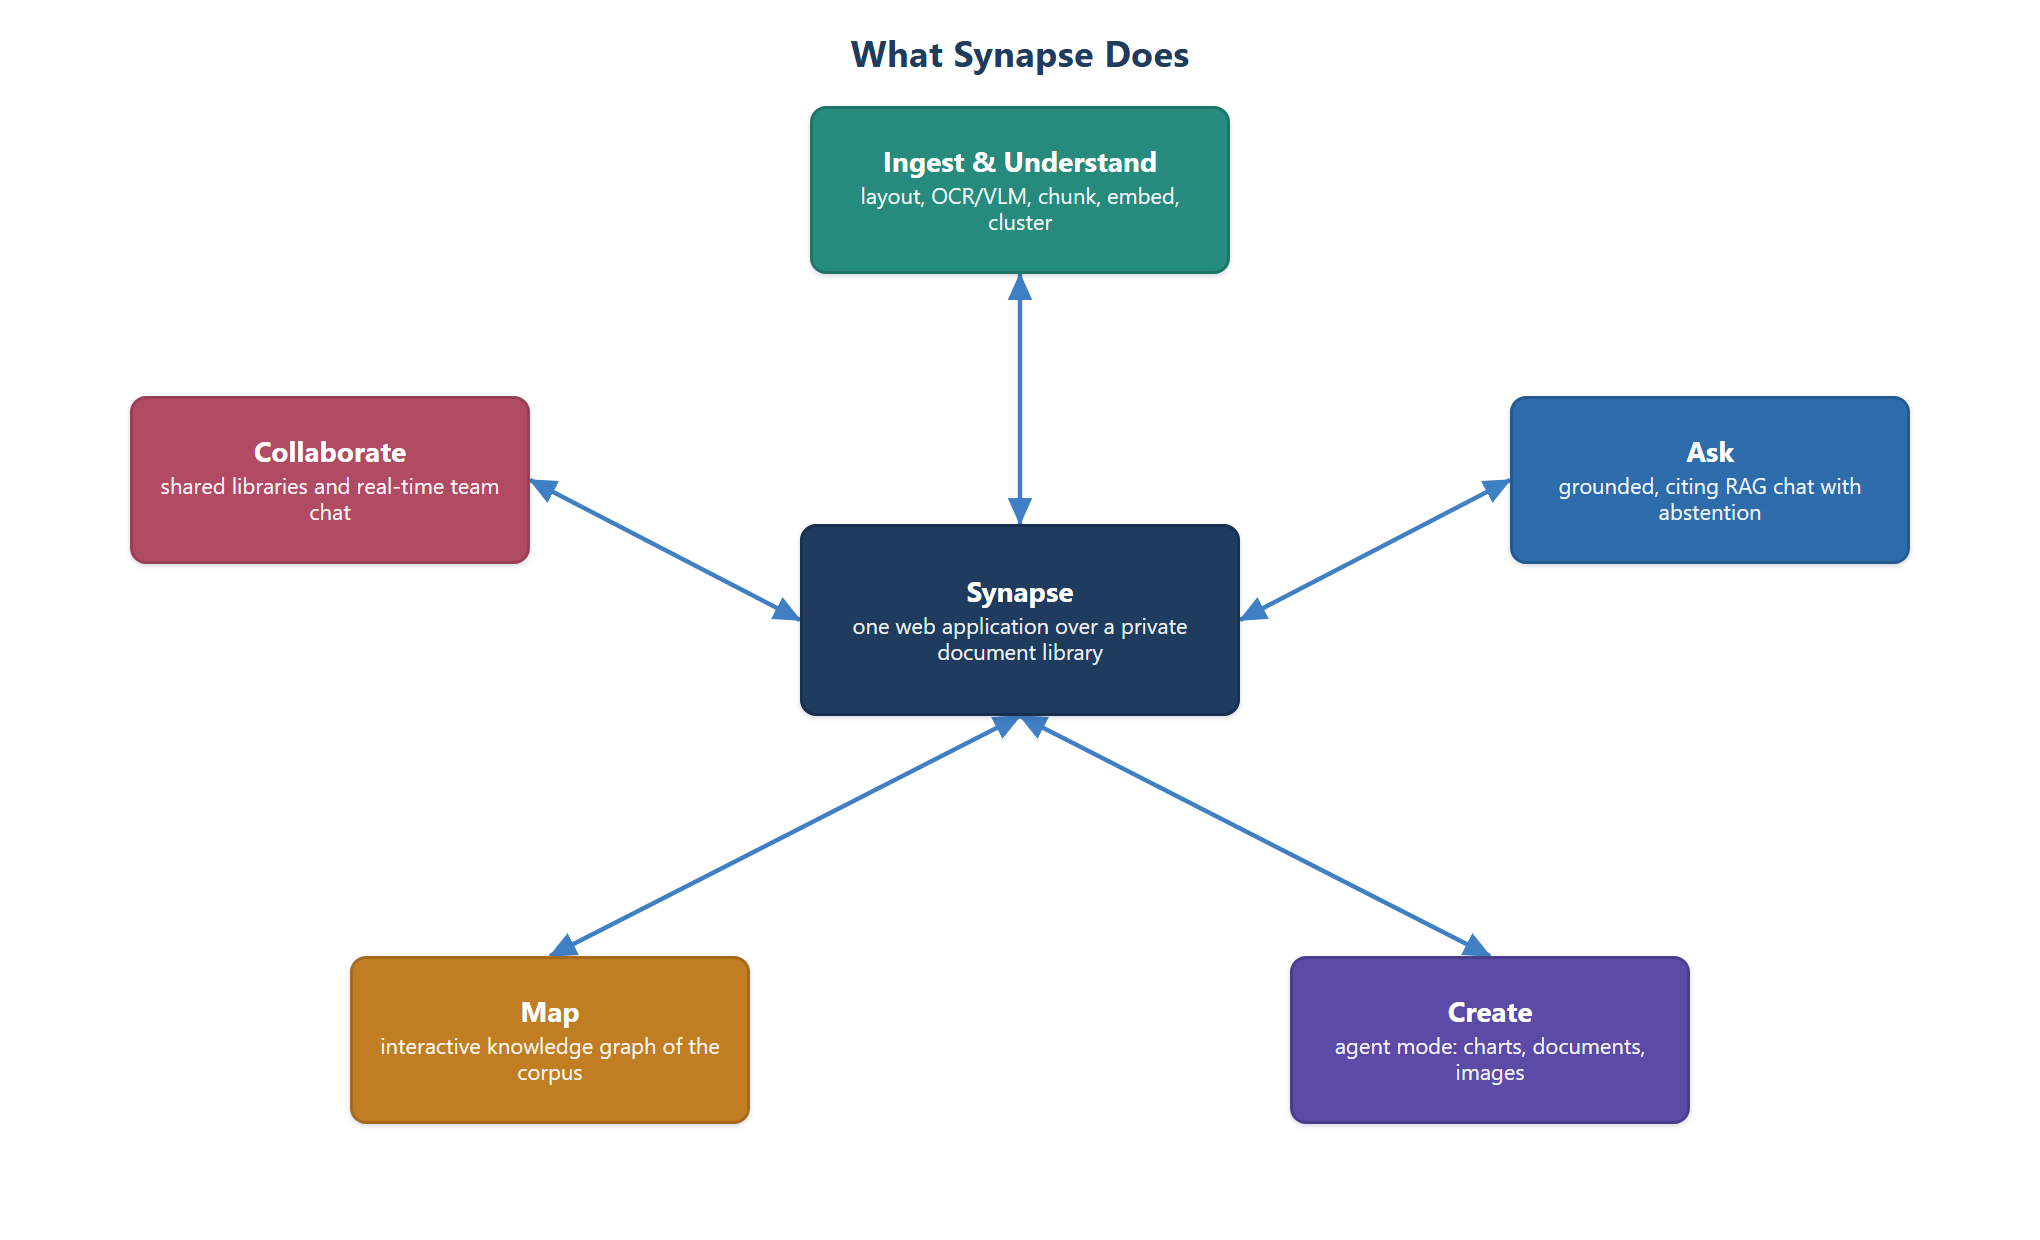
\includegraphics[width=0.92\textwidth]{fig_capabilities.png}
  \caption{The four capabilities Synapse provides over a connected document
  library. A user can ingest and understand a collection, ask grounded
  questions through a citing chat, create artefacts such as charts and
  documents through an agent, and map the corpus as an interactive knowledge
  graph. Teams share these libraries and collaborate in real time. All four
  capabilities act on the same processed library, so work done in one is
  available to the others.}
  \label{fig:capabilities}
\end{figure}

\section{Background and Motivation}

Large language models have made it natural to ask questions in plain language
and receive a fluent reply. On their own, however, these models suffer from two
well-known weaknesses. They only know what was present in their training data,
so they cannot speak about a private contract or an internal report that they
have never seen. And when they are unsure, they tend to answer anyway, producing
confident text that is not supported by any source. For everyday browsing this
is a minor nuisance. For someone deciding on the basis of a legal clause, a
financial figure or a medical guideline, an unsupported answer is worse than no
answer at all.

Retrieval-augmented generation was introduced to address the first weakness
\cite{lewis2020rag}. Instead of relying only on the model's memory, the system
first retrieves passages that are relevant to the question from a trusted
collection, and then asks the model to answer using those passages. This grounds
the reply in real material and makes it possible to show where each statement
came from. Retrieval-augmented generation has become the standard way to build a
question-answering system over a private corpus, and a large body of recent work
has refined how passages are retrieved, judged and combined
\cite{yan2024crag,asai2024selfrag,nguyen2025marag}.

Two practical problems remain, and they motivate this project. The first is that
real document collections are not made of clean paragraphs of text. They contain
scanned pages, spreadsheets, slide decks, figures, tables and source files. A
system that can only read born-digital prose will silently miss much of what a
collection actually holds. The second is that retrieving the right passage is
necessary but not sufficient. A useful system must also judge whether the
retrieved material truly supports an answer, decline to answer when it does not,
and present the result in whatever form the user needs, whether that is a short
written reply, a chart, a document or a picture of how the ideas connect. Synapse
is built around these two concerns.

\section{Problem Statement}

People and teams hold valuable knowledge in large, mixed collections of
documents, but they have no convenient and trustworthy way to use it. General
chatbots cannot read a private library, cannot ground their answers in it, and
will invent facts when the evidence is thin. Traditional search returns a list
of files rather than a direct, supported answer, and neither approach can read a
scanned page, draw a chart from a table, or reveal how the concepts in a
collection relate to one another. What is needed is a single system that ingests
a mixed document collection reliably, answers questions about it with honest,
cited, grounded replies, turns it into useful artefacts on request, and presents
its overall structure in a way a person can explore.

\section{Aim and Objectives}

The aim of this project is to design and build a practical, multi-tenant platform
that lets a user understand, question, visualise and map a private collection of
documents through one web application. To meet this aim, the following objectives
were set.

\begin{enumerate}[leftmargin=*,itemsep=2pt]
  \item To build an ingestion pipeline that reliably processes a mixed
        collection of documents, including born-digital files, scanned pages,
        spreadsheets and source code, into a searchable form.
  \item To design a retrieval-augmented chat that answers questions using only
        the user's library, cites the exact source of every claim, and abstains
        when the evidence is insufficient.
  \item To provide an agent that plans its work, asks for clarification when a
        request is genuinely ambiguous, and produces artefacts such as charts,
        written documents and images from the connected libraries.
  \item To extract the entities and relationships in a processed library and
        present them as an interactive knowledge graph the user can explore.
  \item To support teams, so that several users can share libraries and
        collaborate in real time.
  \item To evaluate the platform on an established document benchmark and on
        purpose-built datasets, and to report retrieval accuracy, answer
        quality, honesty and efficiency.
\end{enumerate}

\section{Scope of the Project}

The project covers the complete platform: the ingestion pipeline, the grounded
chat, the agent, the knowledge graph, team collaboration, and the supporting web
application and infrastructure. The system is multi-tenant, meaning that several
organisations can use it at once with their data kept separate. Documents are
processed automatically, and the user interacts only through the web
application.

The project does not aim to train new language or vision models; it uses
established hosted and open models and concentrates on the design that turns them
into a dependable product. It also does not attempt to be a general web agent
that operates arbitrary external websites; the agent works on the user's own
connected libraries and uploaded files. These boundaries kept the work focused on
the central goal of trustworthy document intelligence over a private collection.

\section{Project Contributions}

The main contributions of this work are as follows. First, it delivers a
single platform that brings together ingestion, grounded question answering,
artefact generation and knowledge mapping over a private library, where most
existing tools address only one of these. Second, it implements a corrective,
multi-agent retrieval loop that grades its own evidence and abstains rather than
guessing, and that attaches a citation to every claim. Third, it implements an
ingestion pipeline that handles scanned and structured documents, not only clean
prose, by combining layout detection, optical character recognition and a
vision-language model. Fourth, it provides an honest evaluation of the platform
on an established benchmark and on purpose-built datasets, reporting not only
accuracy but also how often the system is wrongly confident.

\section{Development Methodology}

The platform was built using an iterative and incremental software lifecycle, as
shown in Figure~\ref{fig:methodology}. Rather than attempting to specify and
build the whole system at once, the work was divided into a sequence of
increments, each adding one coherent piece of functionality such as the
ingestion pipeline, the chat, the agent or the knowledge graph. Every increment
passed through the same short cycle of planning, analysis, design,
implementation, testing and deployment, and produced a working part of the
system that could be tried and reviewed before the next increment began.

\begin{figure}[H]
  \centering
  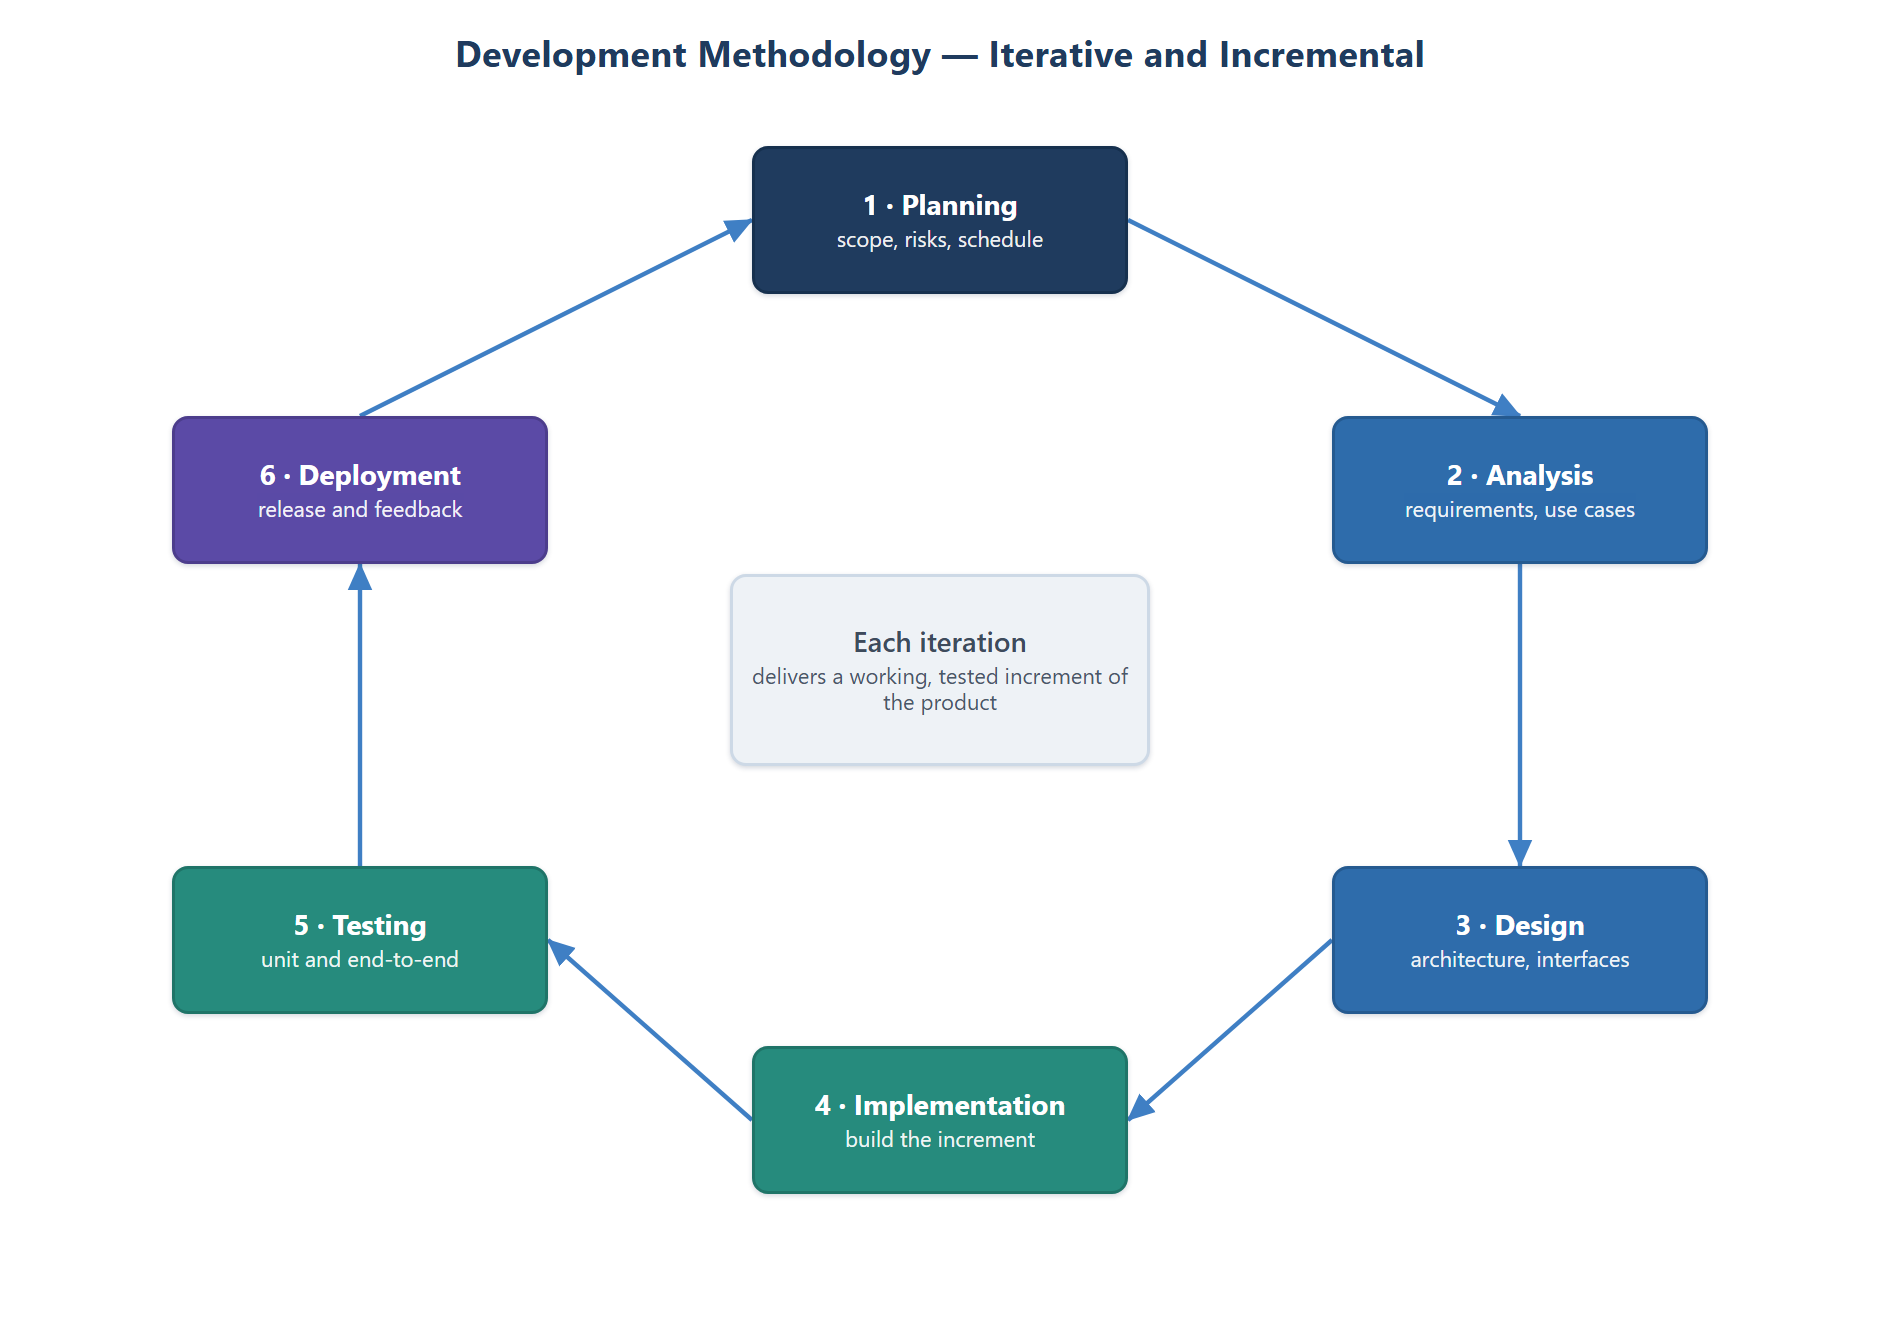
\includegraphics[width=0.78\textwidth]{fig_methodology.png}
  \caption{The iterative and incremental lifecycle followed during development.
  Each feature of the platform passed through the same cycle of planning,
  analysis, design, implementation, testing and deployment. Every iteration
  delivered a working, tested increment, which kept the system usable
  throughout and allowed the design to be corrected early as the requirements
  became clearer.}
  \label{fig:methodology}
\end{figure}

This approach suited the project well. The most uncertain parts, such as how a
scanned page should be read or how the retrieval loop should decide to abstain,
benefited from being tried early on real data and refined in the light of what
worked. Because each increment was integrated into the running system, problems
in the way components fitted together were found while they were still cheap to
fix, and the platform remained demonstrable at every stage.

\section{Organisation of the Thesis}

The remainder of this thesis is organised as follows. Chapter~2 reviews the
related work in retrieval-augmented generation, agents, knowledge graphs and
document understanding, and identifies the gap that Synapse fills.
Chapter~3 presents the requirement analysis, including the use cases and the
functional and non-functional requirements. Chapter~4 describes the design and
architecture of the platform and the main data and control flows. Chapter~5
explains the implementation, covering the technology stack and the principal
modules. Chapter~6 presents the product itself through the web application, using
screenshots of the working system. Chapter~7 reports the testing and evaluation,
including the document benchmark and the purpose-built datasets. Chapter~8
concludes the thesis and outlines directions for future work.

\section{Summary}

This chapter introduced Synapse, a platform that lets a user understand,
question, visualise and map a private collection of documents through one web
application. It explained the motivation, namely that valuable knowledge is
locked inside mixed document collections and that general chatbots can neither
read such a collection nor answer about it honestly. It stated the problem, the
aim and the objectives, set the scope, listed the contributions, and described
the iterative methodology used to build the system. The next chapter reviews the
related work and shows where this project sits within it.

\chapter{Literature Review}
\label{ch:literature}

\section{Introduction}

This chapter reviews the research and systems that Synapse builds upon. It begins
with retrieval-augmented generation, which is the foundation of the grounded
chat, and then looks at the refinements that make retrieval more reliable, such
as self-correction and multi-agent reasoning. It then covers agents that produce
artefacts, knowledge graphs that reveal the structure of a corpus, and the
techniques needed to read documents that are scanned or visually rich. Finally,
it surveys how such systems are evaluated, compares the most relevant systems in
a single table, and identifies the gap that this project fills.

\section{Retrieval-Augmented Generation}

Large language models store a great deal of general knowledge in their
parameters, but that knowledge is fixed at training time and cannot include a
user's private documents. Retrieval-augmented generation, introduced by Lewis et
al.\ \cite{lewis2020rag}, addresses this by attaching a retrieval step to the
model. When a question arrives, the system first finds passages relevant to it
from a trusted collection, and then conditions the model's answer on those
passages. This grounds the answer in real material, allows the source of each
statement to be shown, and lets the knowledge base be updated without retraining
the model.

The quality of the retrieval step is therefore central. Early systems relied on
sparse keyword matching, which is precise for rare terms but misses paraphrases.
Dense passage retrieval \cite{karpukhin2020dpr} instead encodes the question and
the passages as vectors and matches them by meaning, which captures paraphrases
but can drift on exact terms such as names and codes. In practice the two are
complementary, and modern systems combine them. Reciprocal rank fusion
\cite{cormack2009rrf} is a simple and robust way to merge several ranked lists
into one, and is used in Synapse to fuse keyword and vector results. General
purpose text embeddings such as the BGE family \cite{xiao2024cpack} provide the
dense representations, and a cross-encoder reranker re-orders the fused
candidates so that the passages the model finally sees are the most relevant.

\section{Making Retrieval Reliable}

Retrieving relevant passages is necessary but not sufficient. The retrieved
material may still be off-topic, contradictory or simply insufficient, and a
model that answers regardless will produce confident but unsupported text. Two
lines of work address this directly.

Self-RAG \cite{asai2024selfrag} teaches a model to decide when to retrieve, to
criticise its own draft against the retrieved evidence, and to prefer answers
that are well supported. Corrective RAG \cite{yan2024crag} adds a lightweight
evaluator that grades the retrieved set and, when it is weak, triggers a
corrective action such as refining the query or searching more widely before the
answer is composed. Both share a principle that this project adopts: the system
should judge its own evidence and change its behaviour, including declining to
answer, rather than always producing a reply.

A complementary direction breaks the work across several cooperating agents.
MA-RAG \cite{nguyen2025marag} assigns sub-tasks such as planning, retrieval and
synthesis to specialised agents that reason step by step, which helps with
questions that require several pieces of evidence to be combined. Insight-RAG
\cite{pezeshkpour2025insightrag} argues that retrieving on surface similarity
alone can miss the deeper point of a question, and retrieves on the underlying
information need instead. The grounded chat in Synapse follows this overall
shape: it analyses the question, retrieves and grades evidence, and only then
composes a cited answer or abstains.

\section{Agents that Produce Artefacts}

Beyond answering questions, recent agents carry out multi-step tasks. The ReAct
framework \cite{yao2023react} interleaves reasoning and acting, letting a model
think about what to do, take an action, observe the result, and continue. Chain
of thought prompting \cite{wei2022cot} showed that encouraging a model to reason
in explicit steps improves its performance on complex tasks. These ideas underpin
the agent mode in Synapse, which plans its work, decides what data it needs, and
produces an artefact such as a chart or a document.

A practical concern for any agent that reports numbers is faithfulness. If a
model is allowed to write the values inside a chart, it may produce plausible but
incorrect figures. Synapse avoids this by having the agent describe the chart it
wants while the actual data values are bound to it in code from the source file,
so the numbers in an artefact always match the document they came from.

\section{Knowledge Graphs over Documents}

A knowledge graph represents a collection as entities and the relationships
between them, which makes the structure of the collection visible and supports
questions that span several documents. GraphRAG \cite{edge2024graphrag} builds
such a graph from a corpus and uses it to answer broad, summarising questions
that plain passage retrieval handles poorly. CuriousLLM \cite{yang2024curiousllm}
combines graph reasoning with a questioning strategy to improve multi-document
question answering. Synapse includes a knowledge-graph module in the same spirit:
it extracts entities and relationships from a processed library, resolves
duplicates, and presents the result as an interactive graph that keeps a link
from every node and edge back to the passage it came from.

\section{Reading Scanned and Visually Rich Documents}

Real collections are not limited to clean digital text. They include scanned
pages, spreadsheets, slides, figures and tables, and a system that ignores these
will miss much of the content. Document layout analysis locates the regions of a
page, such as paragraphs, tables and figures; DocLayout-YOLO \cite{zhao2024doclayout}
is a recent and efficient model for this task. Optical character recognition then
reads the text inside scanned regions, and modern toolkits such as Surya
\cite{surya2024} handle many languages and layouts. For pages where text alone is
not enough, vision-language models such as Qwen2.5-VL \cite{bai2025qwen25vl} can
read a page image directly and describe its figures and tables. VisDoM
\cite{suri2024visdom} shows the value of treating visually rich elements as
first-class evidence in multi-document question answering. Synapse uses layout
detection, optical character recognition and a vision-language model together so
that scanned and structured documents are processed, not skipped.

\section{Evaluating Document Intelligence}

Measuring these systems is difficult because both retrieval and generation must
be judged, and because a fluent answer is not necessarily a correct one.
Frameworks such as RAGAS \cite{es2024ragas} score properties like faithfulness
and relevance without requiring a hand-written reference for every question.
Because grading free-form answers at scale is costly, a capable model is often
used as an automatic judge \cite{zheng2023judge}, and using more than one judge
helps to expose disagreement. The DOUBLE-BENCH benchmark \cite{shen2025doublebench}
was created specifically to assess document retrieval-augmented generation over
realistic, multimodal documents, with questions that require one or several hops
of reasoning. This project evaluates Synapse on DOUBLE-BENCH together with
purpose-built structured datasets, and reports not only accuracy but also how
often the system is wrongly confident, which is discussed in Chapter~7.

\section{Comparison with Existing Systems}

Table~\ref{tab:comparison} compares Synapse with representative systems across
the capabilities that matter for this project. Most prior systems are strong in
one area, such as corrective retrieval or graph reasoning, but few bring grounded
question answering, artefact generation, knowledge mapping and support for
scanned documents together in a single product that a team can use.

\begin{table}[H]
  \centering
  \caption{Comparison of Synapse with representative related systems. A tick
  means the capability is a designed feature of the system; a dash means it is
  not a focus of that work. Synapse is distinguished by combining grounded,
  abstaining question answering with artefact generation, knowledge mapping and
  support for scanned and structured documents in one platform.}
  \label{tab:comparison}
  \small
  \begin{tabularx}{\textwidth}{Lcccccc}
    \toprule
    \textbf{System} & \textbf{Grounded} & \textbf{Abstains} & \textbf{Multi-} &
    \textbf{Artefact} & \textbf{Knowledge} & \textbf{Scanned/} \\
     & \textbf{QA} & \textbf{when unsure} & \textbf{agent} & \textbf{generation} &
    \textbf{graph} & \textbf{structured} \\
    \midrule
    Classic RAG \cite{lewis2020rag}        & \checkmark & --         & --         & -- & -- & -- \\
    Self-RAG \cite{asai2024selfrag}        & \checkmark & \checkmark & --         & -- & -- & -- \\
    Corrective RAG \cite{yan2024crag}      & \checkmark & \checkmark & --         & -- & -- & -- \\
    MA-RAG \cite{nguyen2025marag}          & \checkmark & \checkmark & \checkmark & -- & -- & -- \\
    GraphRAG \cite{edge2024graphrag}       & \checkmark & --         & --         & -- & \checkmark & -- \\
    VisDoM \cite{suri2024visdom}           & \checkmark & --         & --         & -- & -- & \checkmark \\
    \textbf{Synapse (this work)}           & \checkmark & \checkmark & \checkmark & \checkmark & \checkmark & \checkmark \\
    \bottomrule
  \end{tabularx}
\end{table}

\section{Research Gap}

The review shows steady progress on the individual pieces of document
intelligence, but a gap in how they are brought together. Retrieval has become
more reliable through self-correction and multi-agent reasoning, graphs have made
the structure of a corpus visible, and vision-language models have made scanned
and visually rich pages readable. These advances, however, are usually studied in
isolation and demonstrated on clean benchmarks rather than delivered as a single
product. A user with a real, mixed collection of documents still has no one place
where they can process that collection reliably, ask it questions and receive
honest cited answers, turn it into charts and documents, and explore how its
ideas connect, all while sharing the work with a team.

Synapse addresses this gap. It combines a pipeline that handles scanned and
structured documents, a corrective and multi-agent grounded chat that abstains
when the evidence is insufficient, an agent that produces faithful artefacts, and
an interactive knowledge graph, within one multi-tenant web platform. The
chapters that follow describe its requirements, design, implementation and
evaluation.

\section{Summary}

This chapter reviewed the foundations of the project. It traced retrieval-augmented
generation from its origins to the corrective and multi-agent methods that make
it reliable, surveyed agents that produce artefacts, knowledge graphs over
documents, and the techniques for reading scanned and structured pages, and
looked at how such systems are evaluated. A comparison with representative
systems showed that each addresses part of the problem, and the gap analysis
identified the combined, product-level capability that Synapse provides. The next
chapter sets out the requirements of the system.

\chapter{Requirement Analysis}
\label{ch:requirements}

\section{Introduction}

This chapter sets out what the platform must do. It identifies the people who use
the system, describes the main use cases with a diagram and detailed scenarios,
and then lists the functional and non-functional requirements that guided the
design. The requirements were gathered through the iterative process described in
Chapter~1, refined as each increment was built and tried on real documents.

\section{Stakeholders and Users}

The platform serves two kinds of user and depends on one external party.

\begin{itemize}[leftmargin=*,itemsep=2pt]
  \item \textbf{Member} — a signed-in user who belongs to an organisation. A
        member connects libraries, processes documents, asks questions, generates
        artefacts, explores the knowledge graph and takes part in team chat.
  \item \textbf{Team administrator} — a member with the additional ability to
        manage who belongs to the organisation and what they may access.
  \item \textbf{Model providers} — the external language and vision services
        (OpenAI and OpenRouter) that the platform calls during processing and
        answering. They are not users, but the system depends on them.
\end{itemize}

\section{Use Cases}

Figure~\ref{fig:usecase} shows the principal use cases and the actors that take
part in them. The members carry out the day-to-day work, the team administrator
additionally manages membership and access, and the external model services
participate in answering questions and generating artefacts.

\begin{figure}[H]
  \centering
  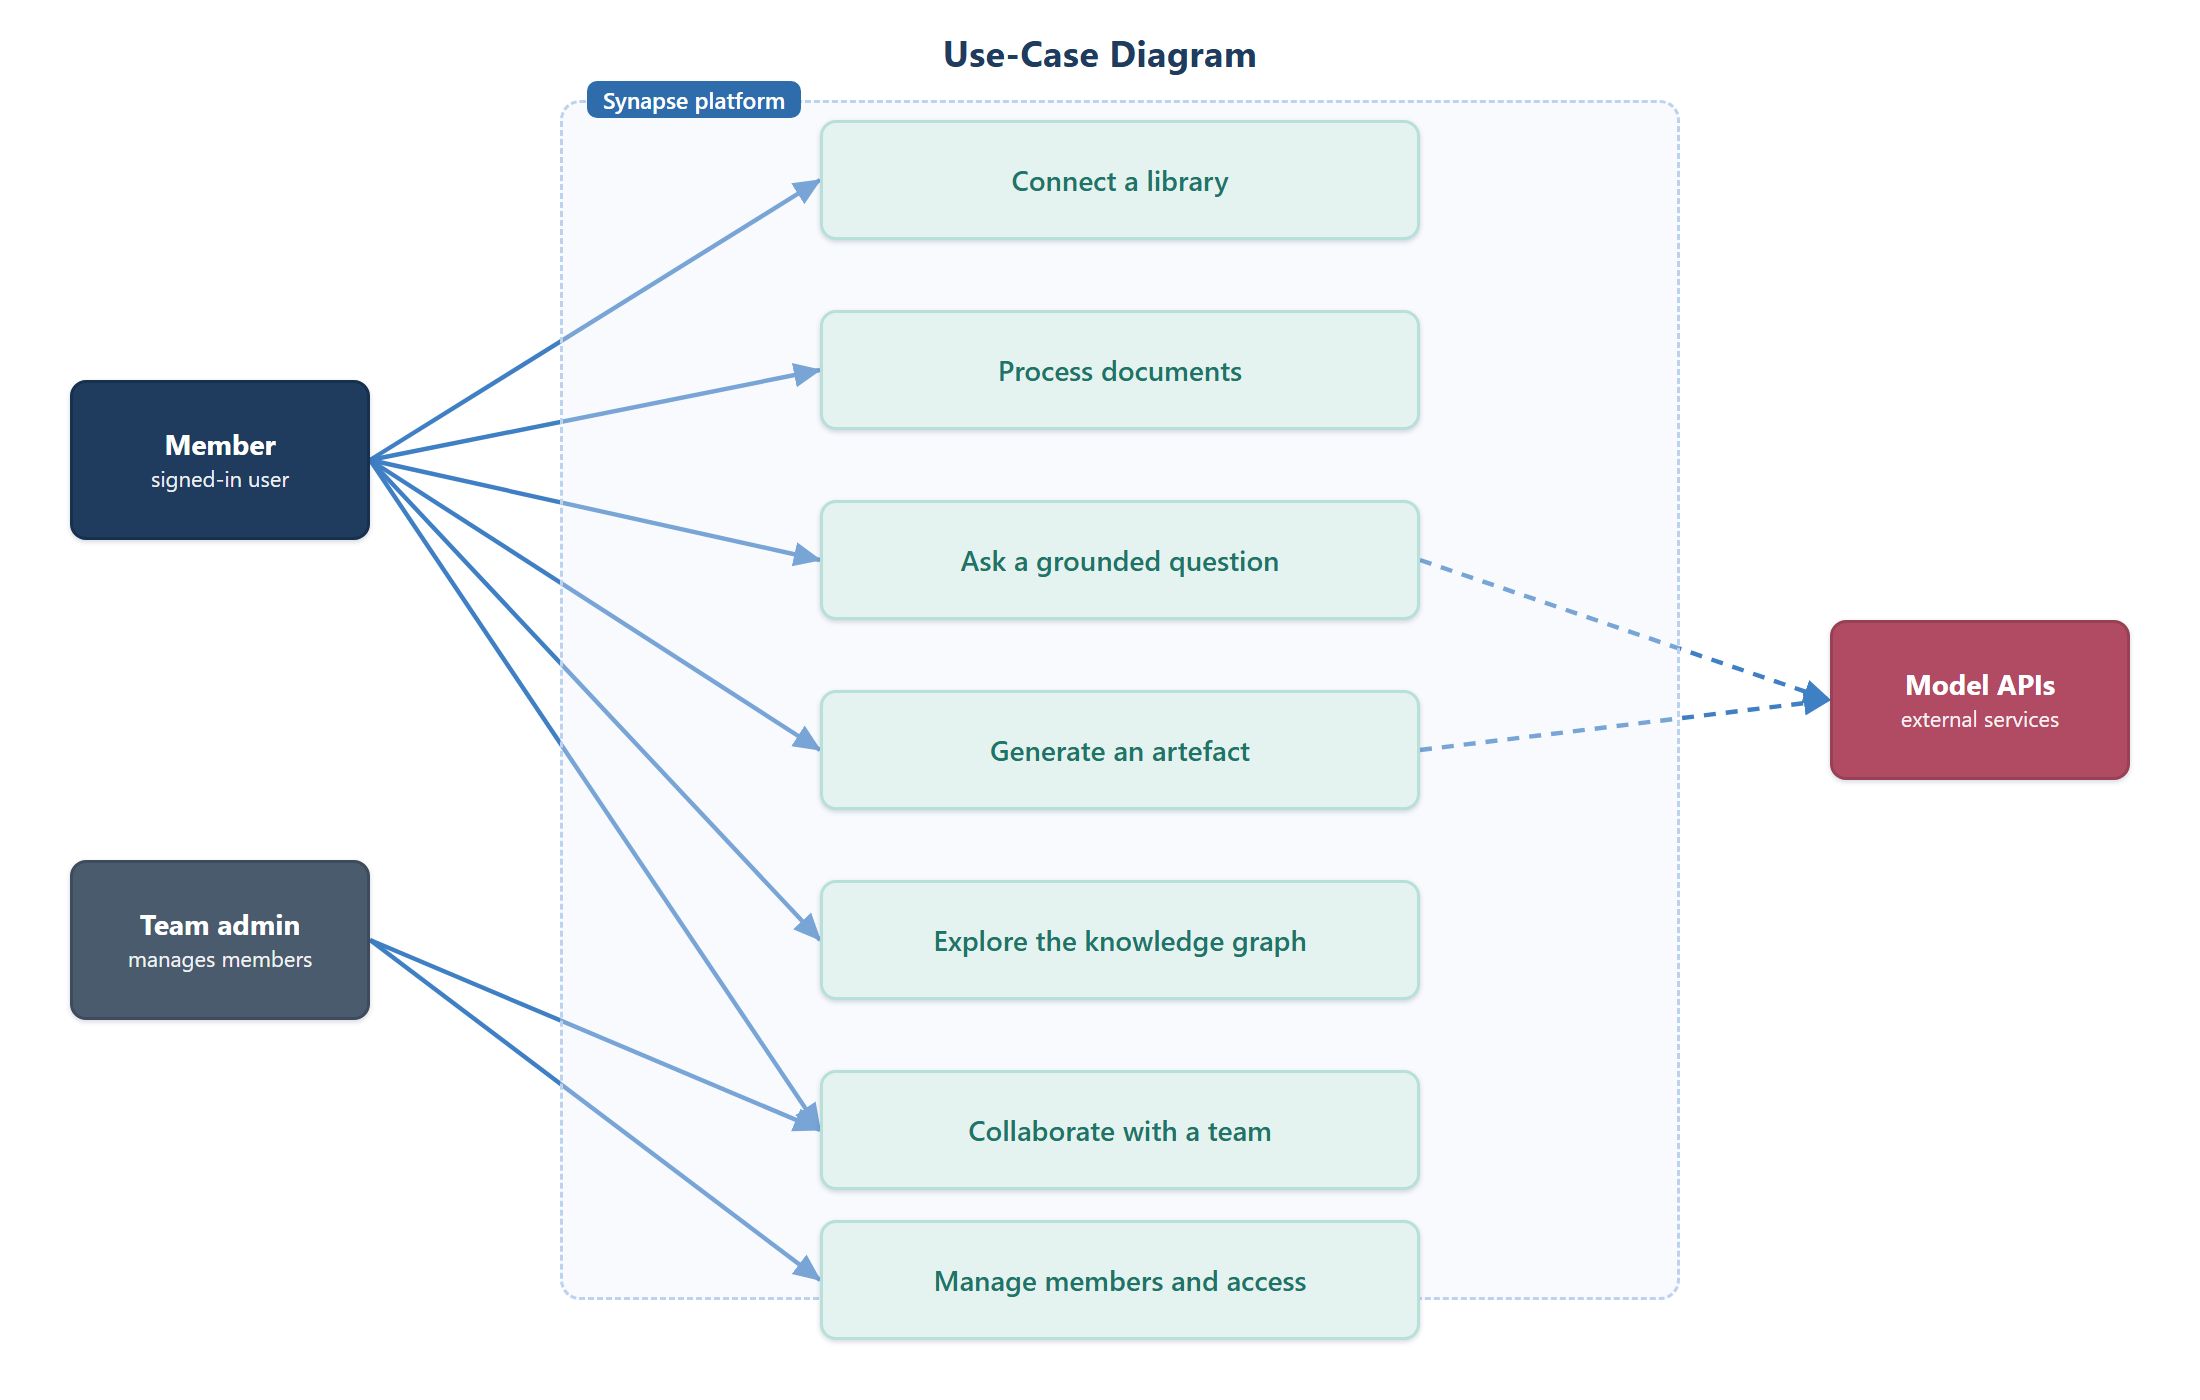
\includegraphics[width=0.96\textwidth]{fig_usecase.png}
  \caption{Use-case diagram of Synapse. A member can connect and process a
  library, ask grounded questions, generate artefacts and explore the knowledge
  graph; a team administrator additionally manages members and access. The
  external model services participate where reasoning over language or images is
  required. All use cases act within the boundary of the platform.}
  \label{fig:usecase}
\end{figure}

The most important use cases are described in detail below. Each scenario lists
the actors, the precondition, the main flow and the result.

\begin{table}[H]
  \centering
  \caption{Use case --- Connect and process a library. This is the entry point
  for all other features: until a library has been processed, there is nothing to
  question, visualise or map. The pipeline runs automatically once a source is
  connected, and the user is shown the progress of each document.}
  \label{tab:uc-ingest}
  \small
  \begin{tabularx}{\textwidth}{@{}p{0.22\textwidth}X@{}}
    \toprule
    \textbf{Use case}      & Connect and process a library \\
    \textbf{Actor}         & Member (primary); model providers (supporting) \\
    \textbf{Precondition}  & The member is signed in and belongs to an organisation. \\
    \midrule
    \textbf{Main flow}     & 1. The member connects a source of documents to a new library. \newline
                             2. The system fetches the files and detects the layout of each page. \newline
                             3. Born-digital text is read directly; scanned pages are read with a vision-language model. \newline
                             4. Figures and tables are captioned, and the text is chunked, embedded and clustered. \newline
                             5. The member sees each document move through the stages to completion. \\
    \textbf{Alternative}   & A document that fails a stage is marked with an error and can be retried without reprocessing the others. \\
    \textbf{Postcondition} & The library is processed and ready to be questioned, visualised and mapped. \\
    \bottomrule
  \end{tabularx}
\end{table}

\begin{table}[H]
  \centering
  \caption{Use case --- Ask a grounded question. This is the most frequent use of
  the platform. The reply is always grounded in the connected library and carries
  a citation for each claim, and the system abstains rather than guessing when the
  evidence is insufficient, which is what makes the answers trustworthy.}
  \label{tab:uc-chat}
  \small
  \begin{tabularx}{\textwidth}{@{}p{0.22\textwidth}X@{}}
    \toprule
    \textbf{Use case}      & Ask a grounded question \\
    \textbf{Actor}         & Member (primary); model providers (supporting) \\
    \textbf{Precondition}  & At least one processed library is selected. \\
    \midrule
    \textbf{Main flow}     & 1. The member types a question in plain language. \newline
                             2. The system analyses the question and retrieves passages by meaning and by keyword, fusing the results. \newline
                             3. It re-ranks the passages and grades whether they are sufficient. \newline
                             4. It composes an answer grounded in the passages, with a citation for each claim. \\
    \textbf{Alternative}   & If the evidence is insufficient, the system says so and does not invent an answer. \\
    \textbf{Postcondition} & The member has a cited answer, or a clear statement that the library cannot support one. \\
    \bottomrule
  \end{tabularx}
\end{table}

\begin{table}[H]
  \centering
  \caption{Use case --- Generate an artefact. The agent turns a request and a set
  of libraries into a chart, document or image. It asks a clarifying question only
  when the request is genuinely ambiguous, and the data in any chart is taken
  directly from the source files so that the figures are faithful.}
  \label{tab:uc-agent}
  \small
  \begin{tabularx}{\textwidth}{@{}p{0.22\textwidth}X@{}}
    \toprule
    \textbf{Use case}      & Generate an artefact \\
    \textbf{Actor}         & Member (primary); model providers (supporting) \\
    \textbf{Precondition}  & A library is selected, or a file is attached to the request. \\
    \midrule
    \textbf{Main flow}     & 1. The member states a goal, such as a chart or a written summary. \newline
                             2. The agent plans the work and decides what data it needs. \newline
                             3. It acquires the data by re-parsing structured files or retrieving from the library. \newline
                             4. It builds the artefact, validates it, renders it interactively and as a file, and explains the result. \\
    \textbf{Alternative}   & If the request is ambiguous, the agent asks a short clarifying question before proceeding. \\
    \textbf{Postcondition} & The member has an artefact they can view and download, with the assumptions noted. \\
    \bottomrule
  \end{tabularx}
\end{table}

\section{Functional Requirements}

Table~\ref{tab:fr} lists the functional requirements. They are grouped by the
feature they belong to, so that the requirements for ingestion, chat, the agent,
the knowledge graph and collaboration can be read together.

\begin{table}[H]
  \centering
  \caption{Functional requirements of the platform, grouped by feature. Together
  they define a system that ingests mixed documents, answers questions with cited
  and honest replies, generates faithful artefacts, maps a corpus as a graph, and
  lets teams collaborate, all within a multi-tenant boundary.}
  \label{tab:fr}
  \small
  \begin{tabularx}{\textwidth}{@{}p{0.10\textwidth}X@{}}
    \toprule
    \textbf{ID} & \textbf{Requirement} \\
    \midrule
    FR-1  & The system shall let a member connect a source and create a library of documents. \\
    FR-2  & The system shall detect page layout and read born-digital text directly. \\
    FR-3  & The system shall read scanned pages using optical character recognition and a vision-language model. \\
    FR-4  & The system shall caption figures and tables, and chunk, embed and cluster the text of each document. \\
    FR-5  & The system shall show the processing status of each document and allow a failed document to be retried. \\
    FR-6  & The system shall answer a plain-language question using only the selected libraries. \\
    FR-7  & The system shall retrieve evidence by combining vector and keyword search and shall re-rank the results. \\
    FR-8  & The system shall attach a citation to the source passage for every claim in an answer. \\
    FR-9  & The system shall abstain when the retrieved evidence is insufficient to support an answer. \\
    FR-10 & The system shall let a member request an artefact and shall ask a clarifying question only when the request is ambiguous. \\
    FR-11 & The system shall generate interactive charts and diagrams, written documents, and images, each downloadable as a file. \\
    FR-12 & The system shall take chart values directly from the source data so that artefacts are faithful. \\
    FR-13 & The system shall extract entities and relationships from a processed library and present them as an interactive knowledge graph. \\
    FR-14 & The system shall keep a link from each graph node and edge back to its source passage. \\
    FR-15 & The system shall let members of an organisation share libraries and chat together in real time. \\
    FR-16 & The system shall let a team administrator manage members and their access. \\
    FR-17 & The system shall keep each organisation's data separate from every other organisation's data. \\
  \end{tabularx}
\end{table}

\section{Non-Functional Requirements}

Table~\ref{tab:nfr} lists the non-functional requirements, which describe how
well the system must behave rather than what it must do. They cover performance,
reliability, security and privacy, scalability, usability and maintainability.

\begin{table}[H]
  \centering
  \caption{Non-functional requirements. These qualities were treated as
  first-class goals: honesty and privacy in particular shaped the design of the
  retrieval loop and the multi-tenant data model described in later chapters.}
  \label{tab:nfr}
  \small
  \begin{tabularx}{\textwidth}{@{}p{0.10\textwidth}p{0.24\textwidth}X@{}}
    \toprule
    \textbf{ID} & \textbf{Quality} & \textbf{Requirement} \\
    \midrule
    NFR-1 & Performance     & A typical question should return its first evidence within a few seconds, and a full answer within the time a user will reasonably wait. \\
    NFR-2 & Reliability     & Document processing shall be resumable, so that a failure in one stage or document does not lose the work already done. \\
    NFR-3 & Honesty         & The system shall prefer to abstain over giving an unsupported answer, and shall make its citations checkable. \\
    NFR-4 & Security \& privacy & Each organisation's documents and conversations shall be accessible only to its members, enforced at the database. \\
    NFR-5 & Scalability     & The processing pipeline shall handle large libraries by working in batches rather than all at once. \\
    NFR-6 & Usability       & A member shall be able to use every feature through the web application without technical knowledge. \\
    NFR-7 & Maintainability & The system shall be built from small, well-separated modules so that features can evolve independently. \\
  \end{tabularx}
\end{table}

\section{Assumptions and Constraints}

The platform assumes that documents are provided in common formats and that the
external model services are available, since processing and answering depend on
them. It is constrained to use established hosted and open models rather than
training new ones, and the graphics-intensive processing runs on a single
GPU-equipped server, which sets a practical bound on how much work can be in
progress at once. These assumptions match the scope set in Chapter~1.

\section{Summary}

This chapter identified the users of the platform, presented the main use cases
through a diagram and detailed scenarios, and set out seventeen functional and
seven non-functional requirements. Honesty and privacy were highlighted as
qualities that would shape the design. The next chapter turns these requirements
into a concrete design and architecture.

\chapter{Design and Architecture}
\label{ch:design}

\section{Introduction}

This chapter describes how the platform is put together. It begins with the
overall architecture and the principles that guided it, then explains the design
of each major subsystem: the grounded chat, the agent, and the knowledge graph.
It then presents the data model that ties everything together and the way the
system is deployed. The implementation detail that realises this design is the
subject of Chapter~5.

\section{Architectural Overview}

Synapse is organised into tiers, as shown in Figure~\ref{fig:architecture}. The
web application runs in the browser and talks to a Cloudflare Worker, which hosts
the application at the edge and forwards requests to the backend. The backend is a
FastAPI service running on a GPU-equipped server, and it is where the real work
happens: an API layer receives requests, a pool of workers processes documents
through the pipeline, a retrieval and reasoning component answers questions, and a
knowledge-graph builder constructs the graph. These components share two stores,
a Supabase database with vector search for text and embeddings and a Cloudflare
R2 bucket for files and artefacts, and they call external model services for
language and vision tasks.

\begin{figure}[H]
  \centering
  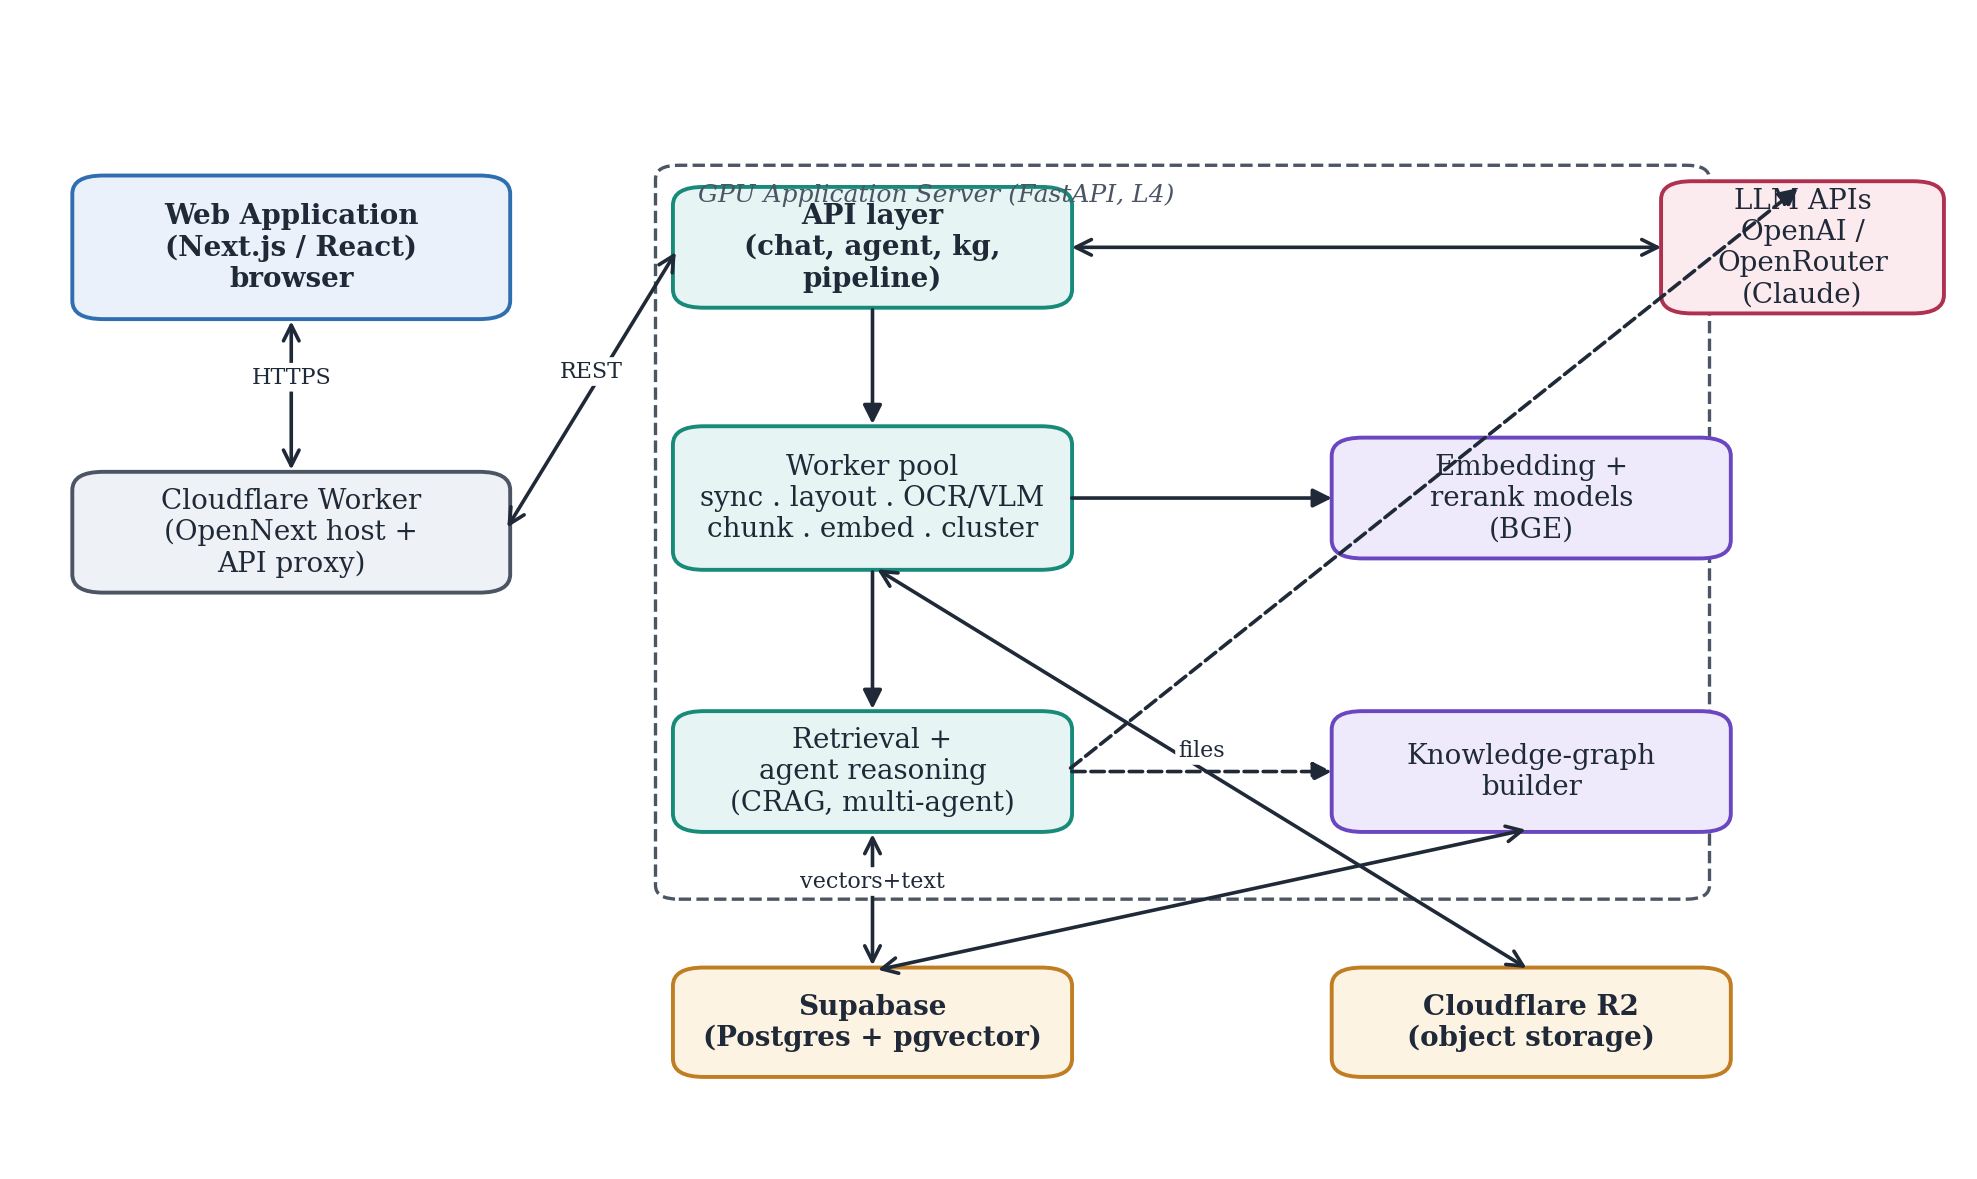
\includegraphics[width=\textwidth]{fig_architecture.png}
  \caption{High-level architecture of Synapse. The browser talks to a Cloudflare
  Worker that hosts the application and proxies to a FastAPI service on a
  GPU server. The backend separates the API layer, the document workers, the
  retrieval and reasoning component and the knowledge-graph builder, all sharing a
  Supabase database and an R2 object store and calling external model services.
  This separation lets each concern scale and evolve on its own.}
  \label{fig:architecture}
\end{figure}

\section{Design Principles}

A small number of principles shaped the design. The first is \emph{grounding}:
every answer must be traceable to a source passage, and the system must be able to
say it does not know. The second is \emph{separation of concerns}: ingestion,
retrieval, artefact generation and graph construction are independent components
with clear interfaces, which kept each one simple and allowed them to be built and
tested in turn. The third is \emph{resumable processing}: documents move through
the pipeline in stages that can be retried, so a failure never discards completed
work. The fourth is \emph{tenant isolation}: every piece of data belongs to an
organisation, and access is enforced at the database rather than trusted to the
application. These principles recur throughout the subsystems described below.

\section{The Grounded Chat Subsystem}

The grounded chat answers questions using only the user's selected libraries.
Its design, shown in Figure~\ref{fig:chatflow}, follows the corrective and
multi-agent ideas from Chapter~2. A question is first analysed and, where useful,
rewritten and expanded so that retrieval has the best chance of finding the right
passages. Retrieval is hybrid: a vector search finds passages by meaning and a
keyword search finds them by exact terms, and the two ranked lists are fused. The
fused candidates are re-ranked by a cross-encoder, and the top passages are graded
for relevance and sufficiency. Only if the evidence is sufficient does the system
compose an answer, attaching a citation to each claim; otherwise it abstains and
says the library cannot support an answer.

\begin{figure}[H]
  \centering
  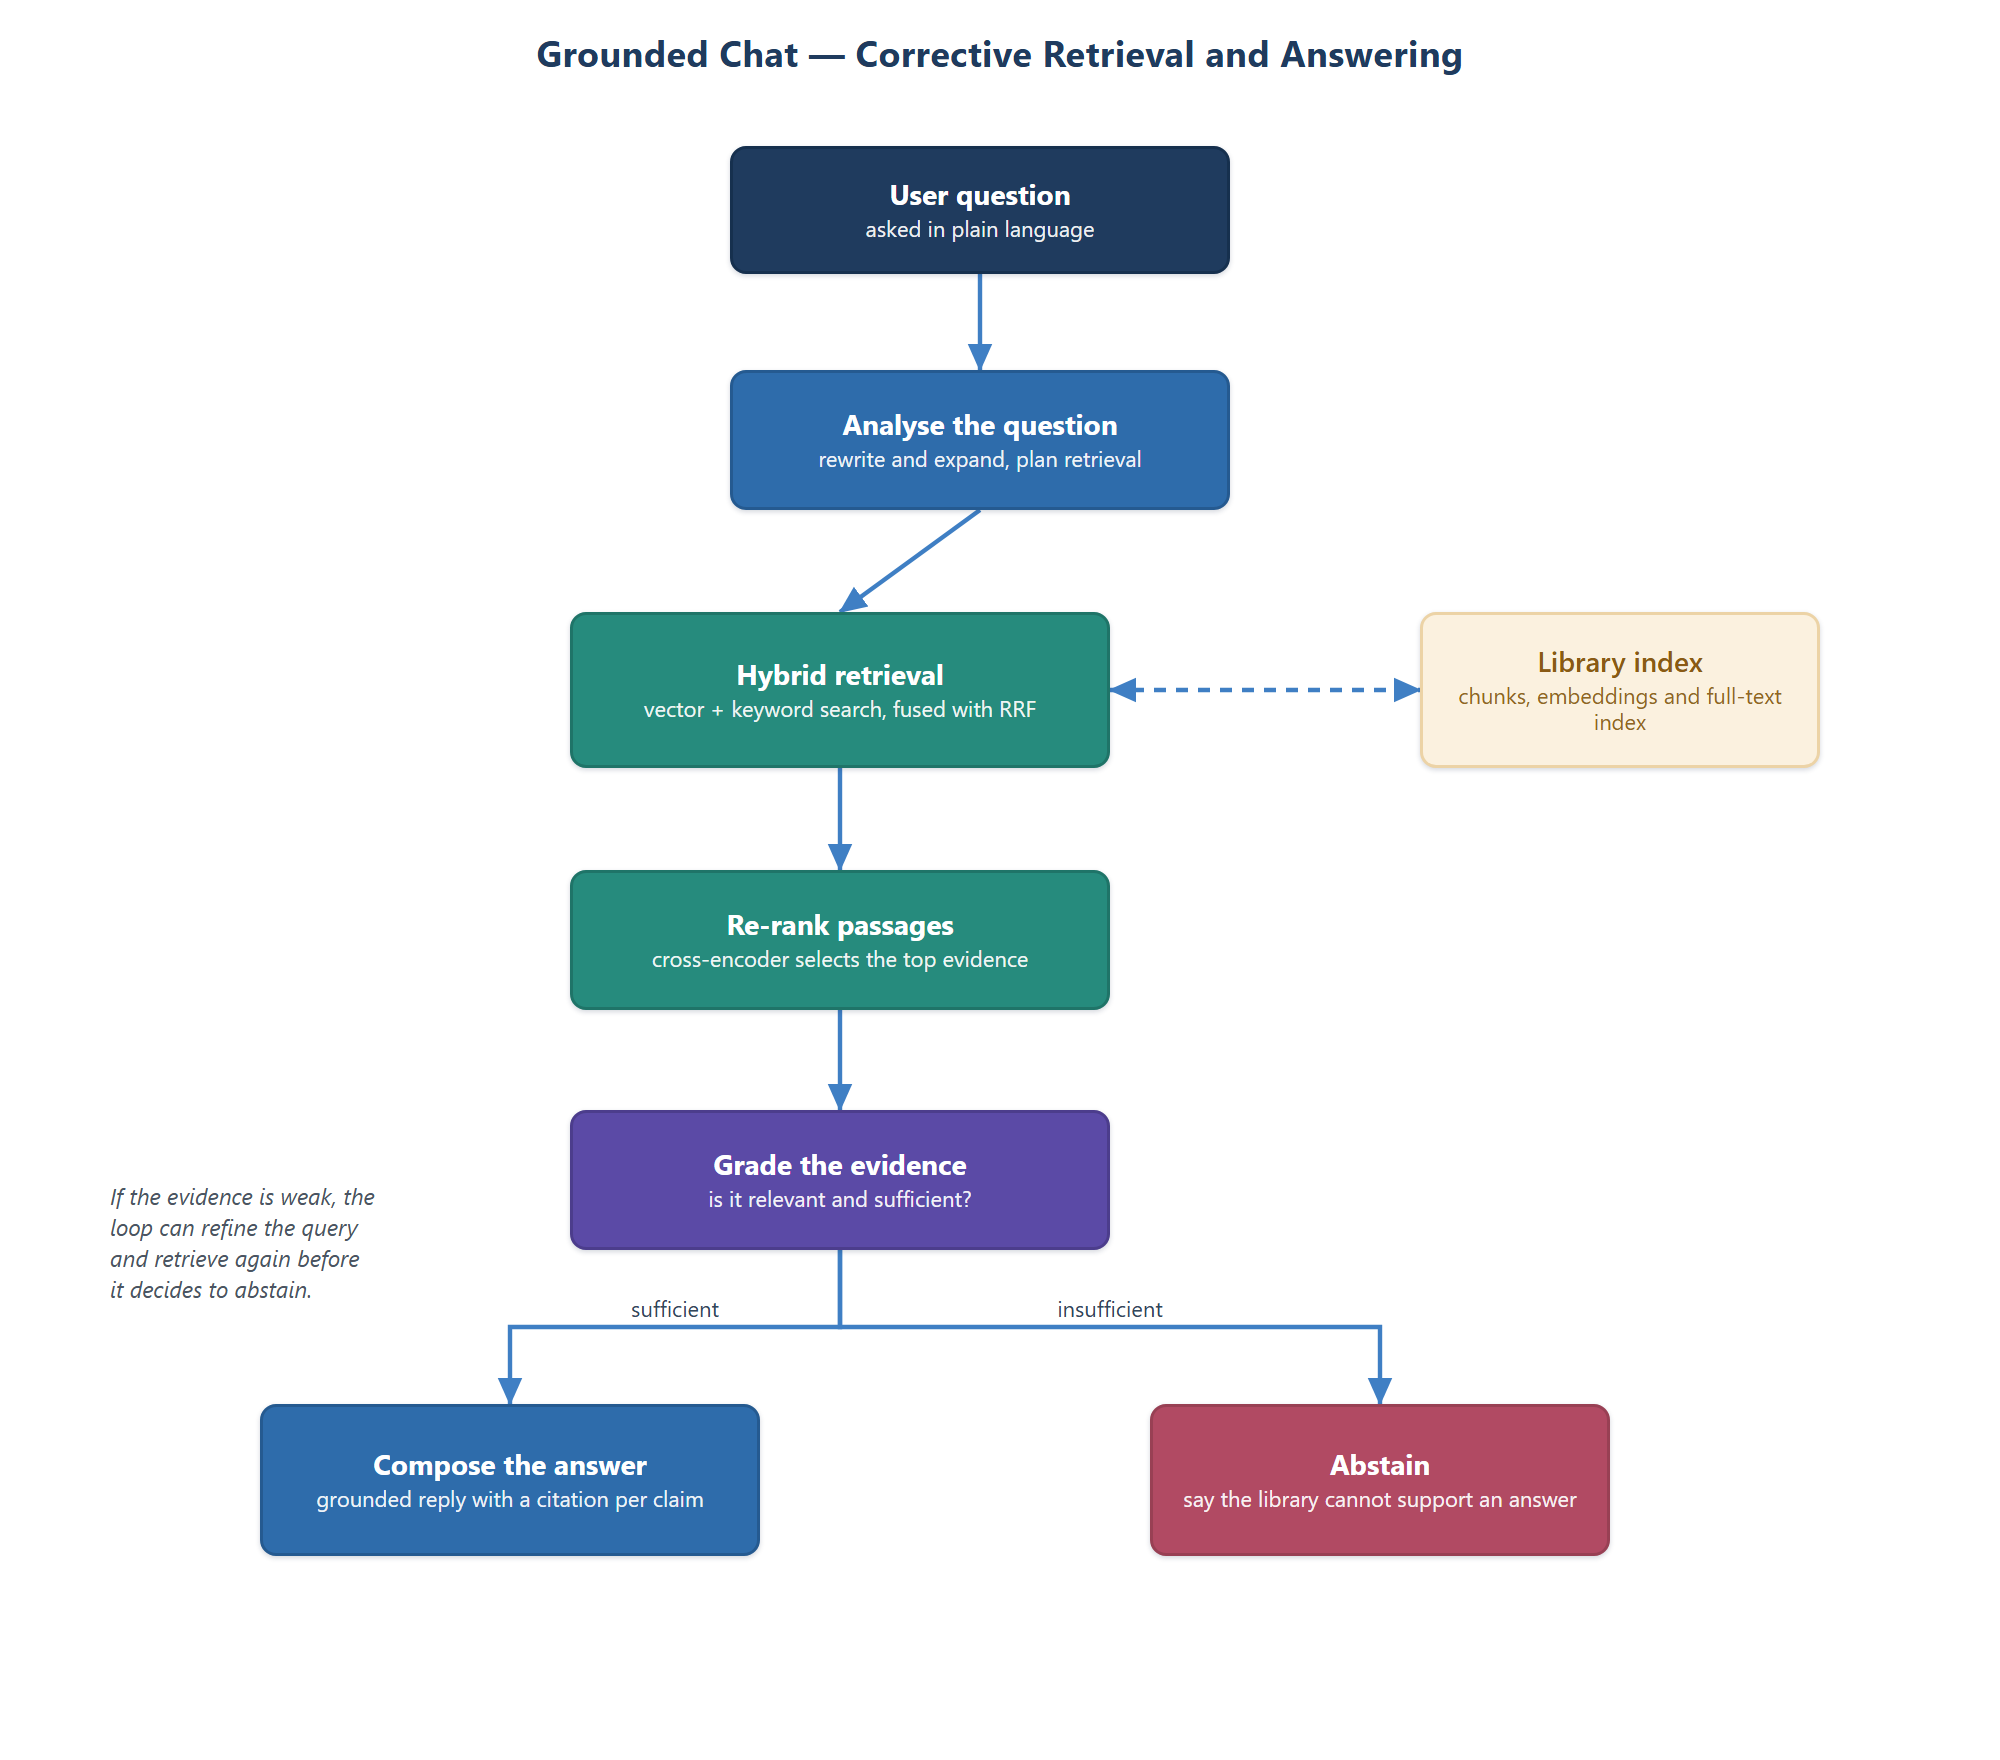
\includegraphics[width=0.62\textwidth]{fig_chat_flow.png}
  \caption{Design of the grounded chat. The question is analysed, evidence is
  retrieved by both meaning and keyword and then re-ranked, and the evidence is
  graded before any answer is written. A sufficient set of passages leads to a
  cited answer; an insufficient set leads the system to abstain rather than guess.
  This grade-then-answer order is what keeps the replies honest.}
  \label{fig:chatflow}
\end{figure}

This design directly serves the honesty requirement. Because the decision to
answer is made after the evidence has been graded, the system can decline cleanly,
and because each claim is tied to a passage, a reader can verify the answer
against the source.

\section{The Agent Subsystem}

The agent turns a goal and a set of libraries into an artefact such as a chart, a
document or an image. Its design is shown in Figure~\ref{fig:agentflow}. The agent
first plans the work, deciding what the user wants and what data is required. If
the request is genuinely ambiguous it asks a single clarifying question;
otherwise it proceeds and records the assumptions it has made. It then acquires
the data, either by re-parsing a structured file exactly or by retrieving from the
library, builds a specification of the artefact, validates and if necessary
repairs it, renders it both interactively and as a downloadable file, and finally
explains the result.

\begin{figure}[H]
  \centering
  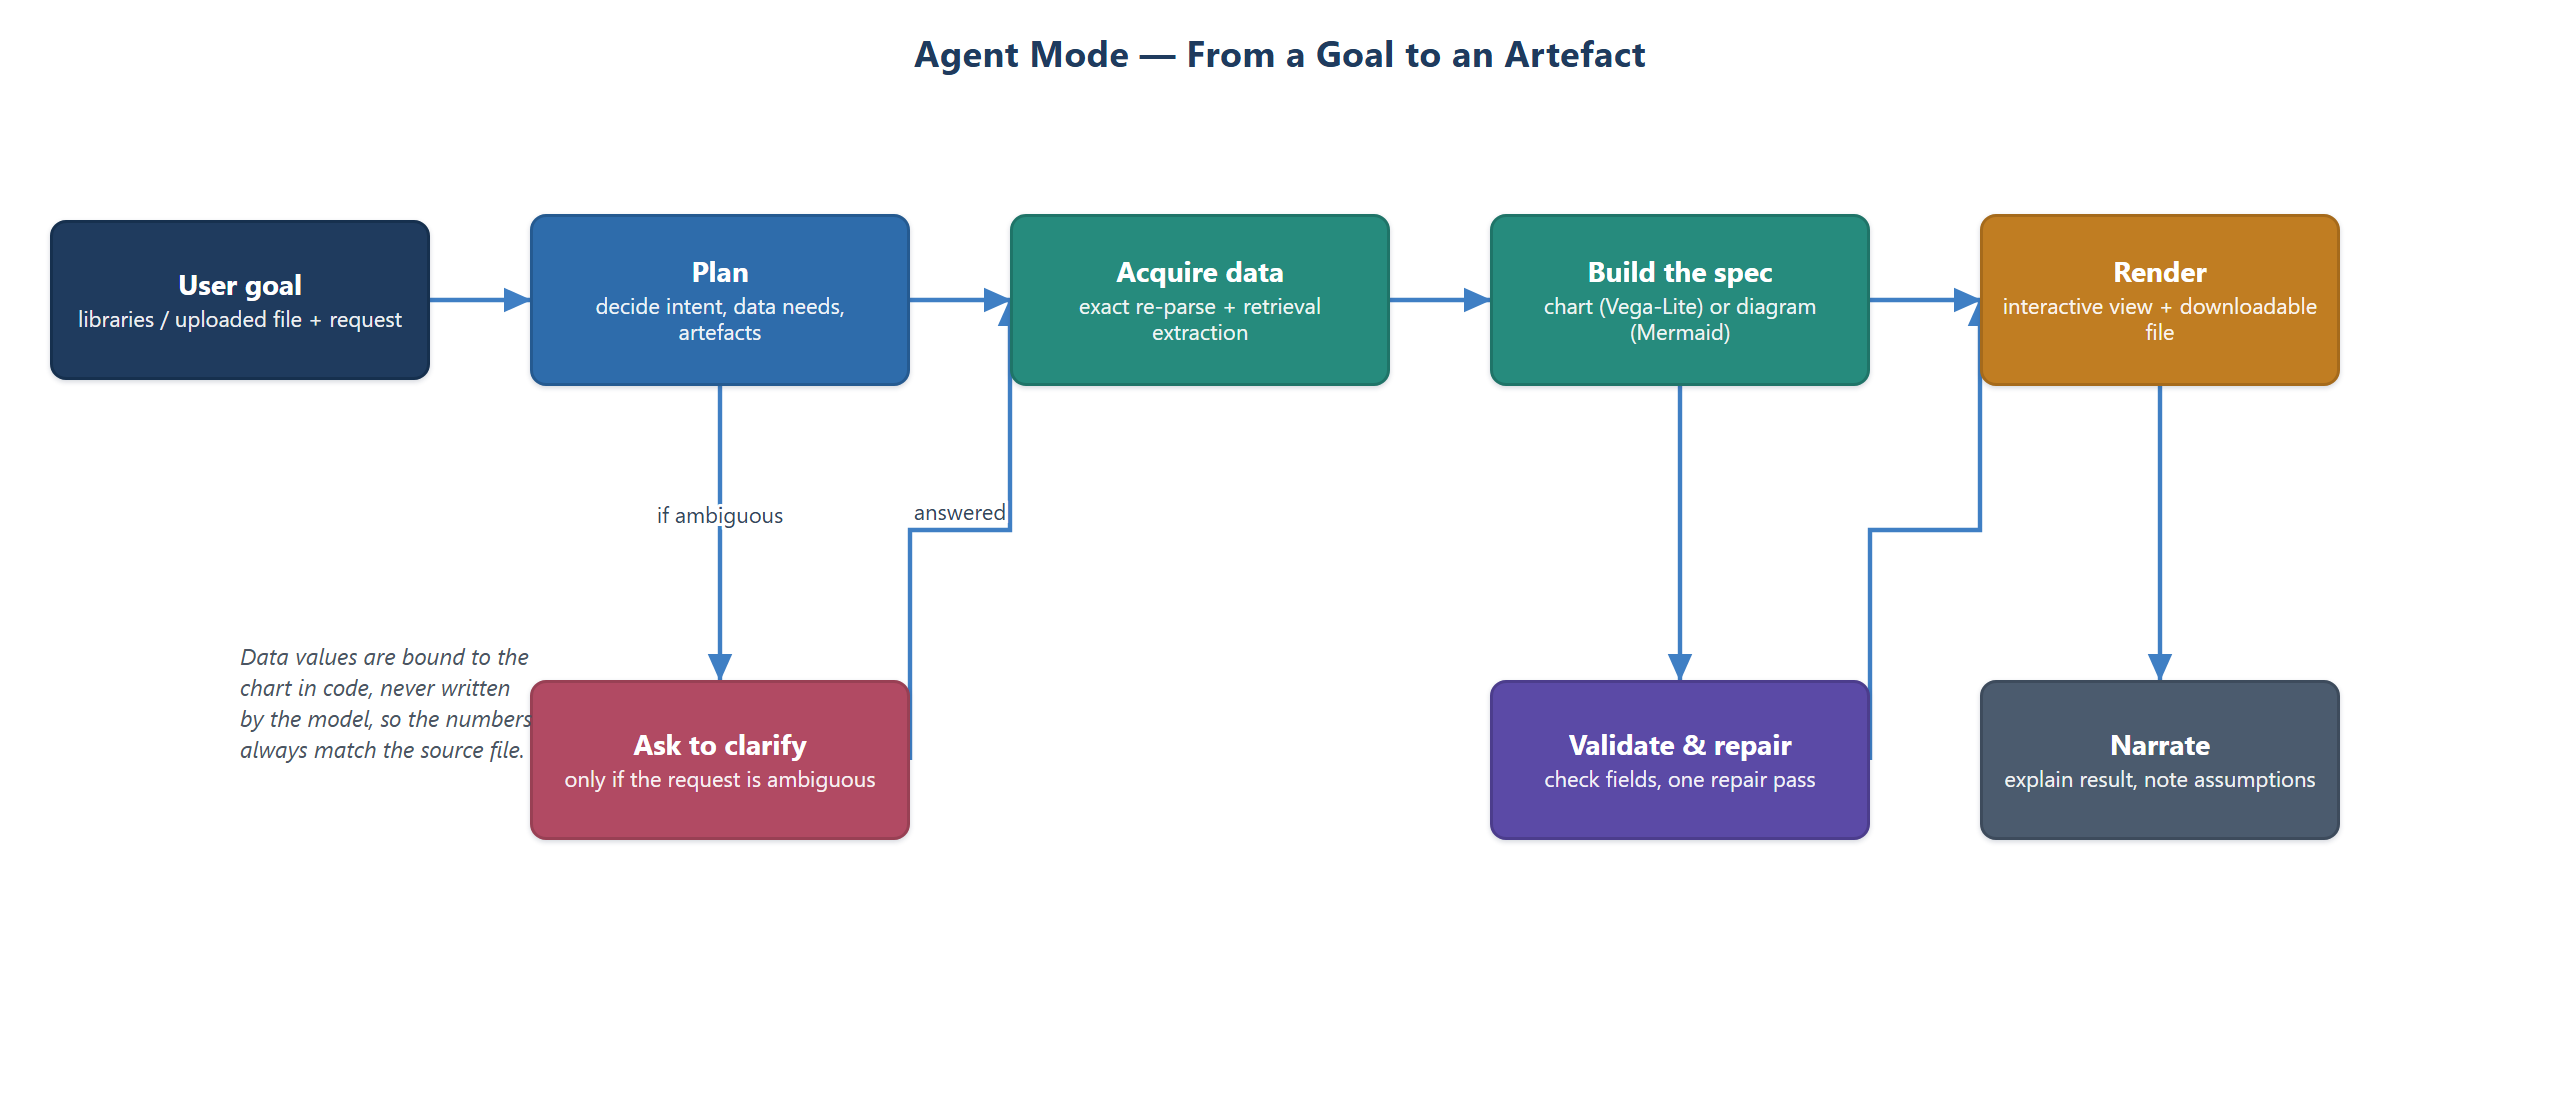
\includegraphics[width=\textwidth]{fig_agent_flow.png}
  \caption{Design of the agent. A goal is planned into data needs and artefacts;
  the agent clarifies only when the request is ambiguous, acquires the data,
  builds and validates a specification, and renders the artefact for viewing and
  download. The data values are bound to a chart in code rather than written by
  the model, so the figures always match the source document.}
  \label{fig:agentflow}
\end{figure}

The key design decision here is the separation between describing an artefact and
filling it with data. The model proposes the shape of a chart, but the numbers are
bound to it from the source file in code. This keeps the artefacts faithful, which
is essential if a user is to rely on them.

\section{The Knowledge-Graph Subsystem}

The knowledge-graph subsystem reveals how the ideas in a library relate. Its
construction is shown in Figure~\ref{fig:kgbuild}. Starting from the processed
library, it extracts entities and relationships from each chunk using a language
model, resolves duplicate entities so that the same thing mentioned in different
ways becomes a single node, builds the graph by assembling the nodes and edges and
weighting them, and serves the result as an interactive graph in the web
application. Every node and edge keeps a link back to the passage it came from, so
the graph is not only a picture but also a way back into the evidence.

\begin{figure}[H]
  \centering
  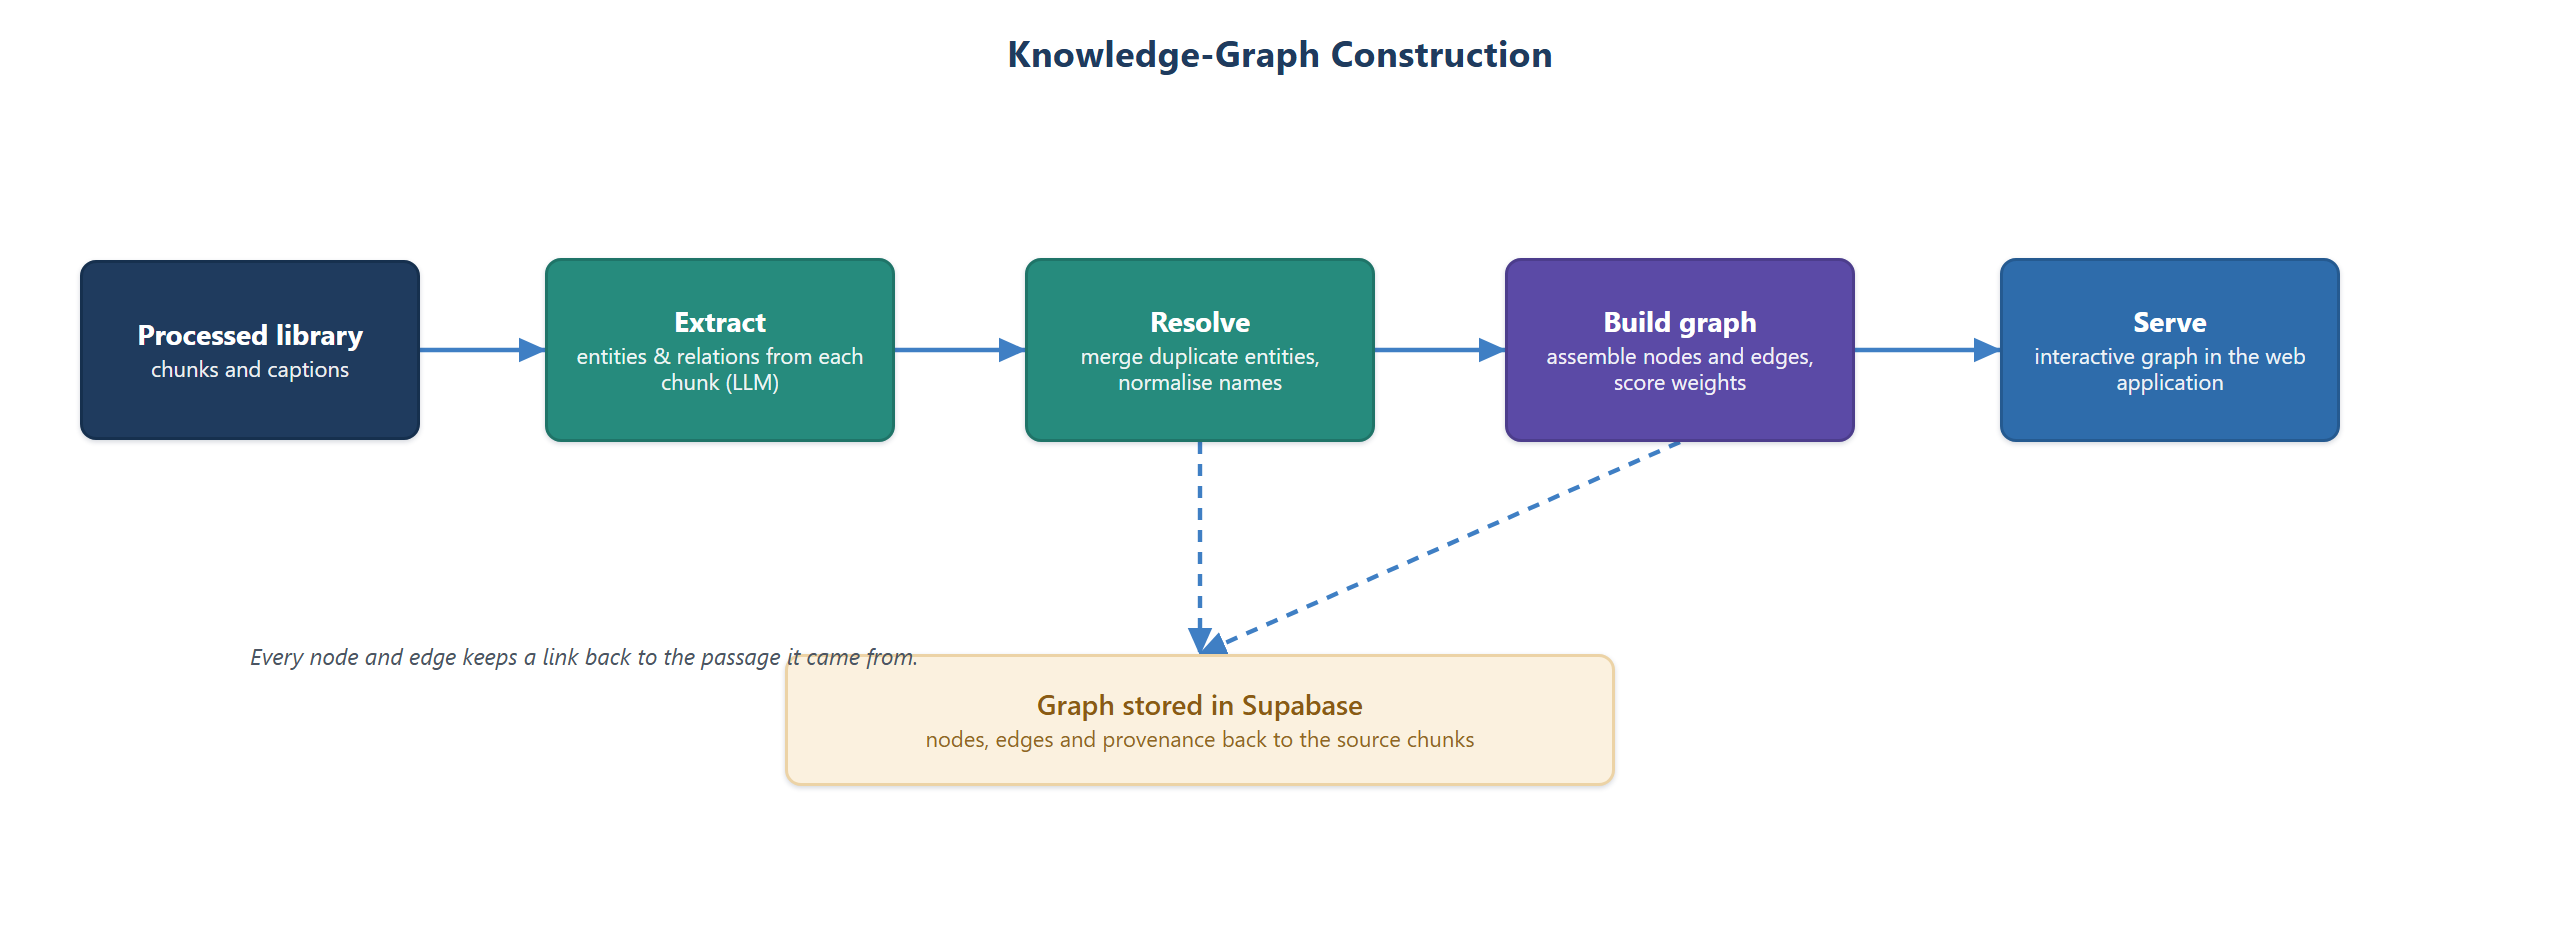
\includegraphics[width=\textwidth]{fig_kg_build.png}
  \caption{Design of the knowledge-graph subsystem. Entities and relationships are
  extracted from each chunk, duplicate entities are resolved into single nodes, the
  graph is assembled and weighted, and it is served interactively. Provenance is
  kept throughout, so a user can move from a node or edge back to the source
  passage that supports it.}
  \label{fig:kgbuild}
\end{figure}

\section{Data Model}

The data model, shown in Figure~\ref{fig:datamodel}, ties the subsystems together.
At its centre is the organisation, which is the tenant boundary; users belong to an
organisation, and libraries are owned by it. A library contains documents, and each
document is split into chunks that carry both their text and their embedding, which
is what retrieval searches. Conversations and their messages, and the nodes and
edges of the knowledge graph, are likewise attached to the organisation. Every row
is scoped to an organisation, and access is enforced by row-level security in the
database, which is how tenant isolation is guaranteed.

\begin{figure}[H]
  \centering
  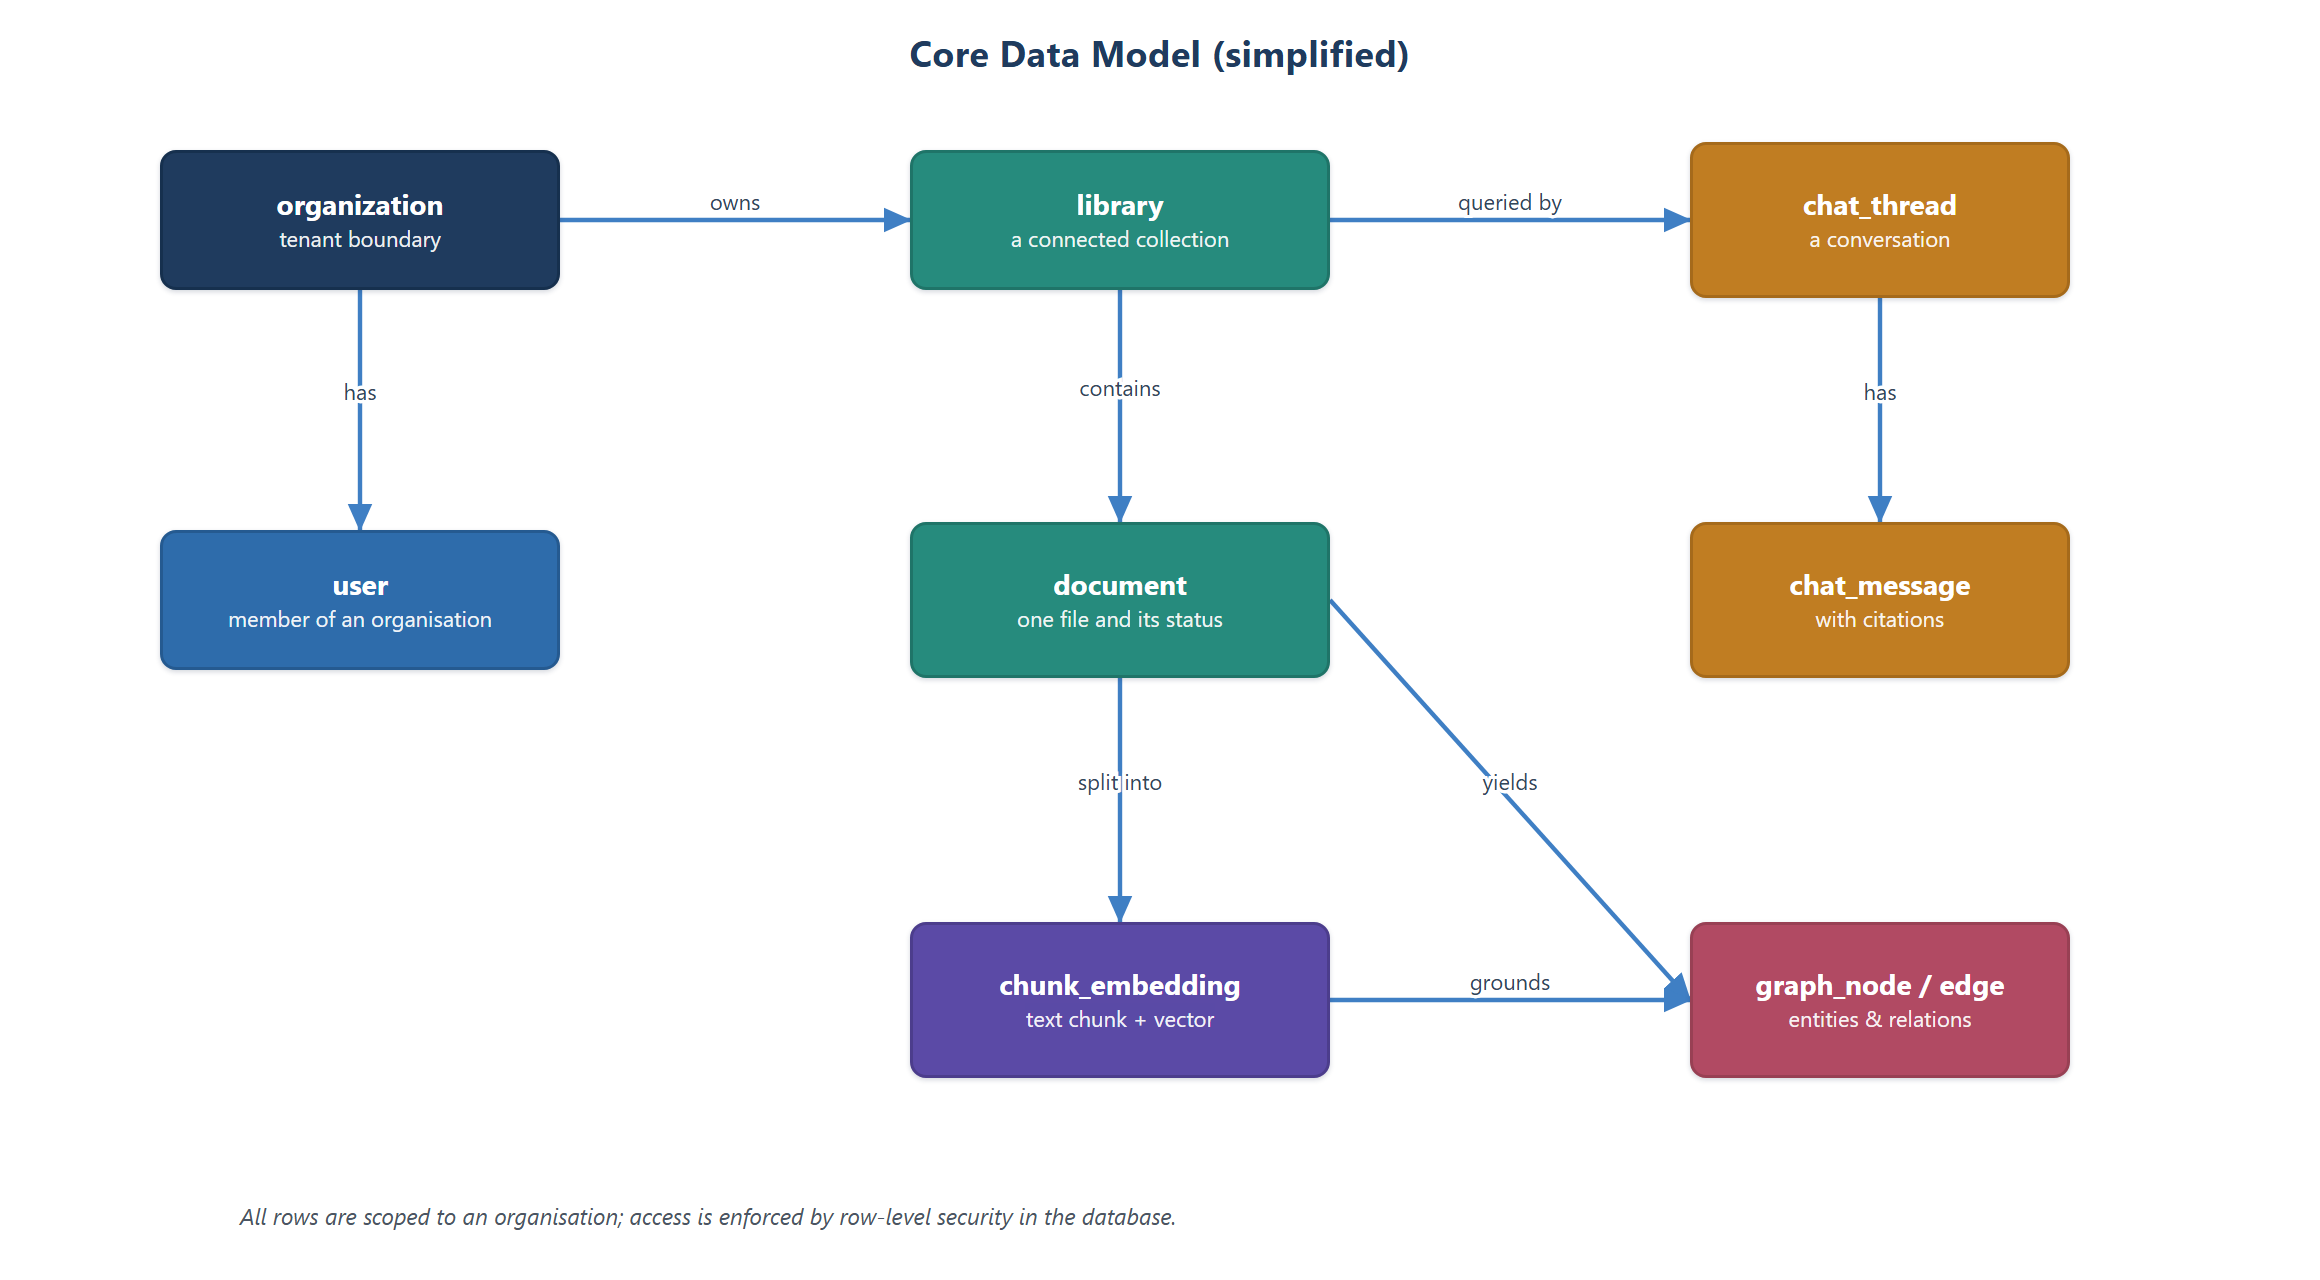
\includegraphics[width=\textwidth]{fig_data_model.png}
  \caption{Simplified core data model. The organisation is the tenant boundary;
  users, libraries, documents, chunks, conversations and graph elements all belong
  to it. Chunks carry the embeddings that retrieval searches, and the graph
  elements are grounded in the same chunks, so the data model supports both
  answering and mapping from one consistent structure.}
  \label{fig:datamodel}
\end{figure}

\section{Deployment Architecture}

Figure~\ref{fig:deployment} shows how the parts are deployed. The web application
is served from a Cloudflare Worker, with files and artefacts in an R2 bucket and
live updates delivered over a realtime channel. The heavy processing runs on a
single GPU-equipped virtual machine that hosts the FastAPI service, the pipeline
workers and the local embedding and reranking models. The database, with its
vector search, is a managed Supabase instance, and the language and vision models
are reached over the network. This arrangement keeps the user-facing parts fast
and close to the user while concentrating the graphics-intensive work on one
server.

\begin{figure}[H]
  \centering
  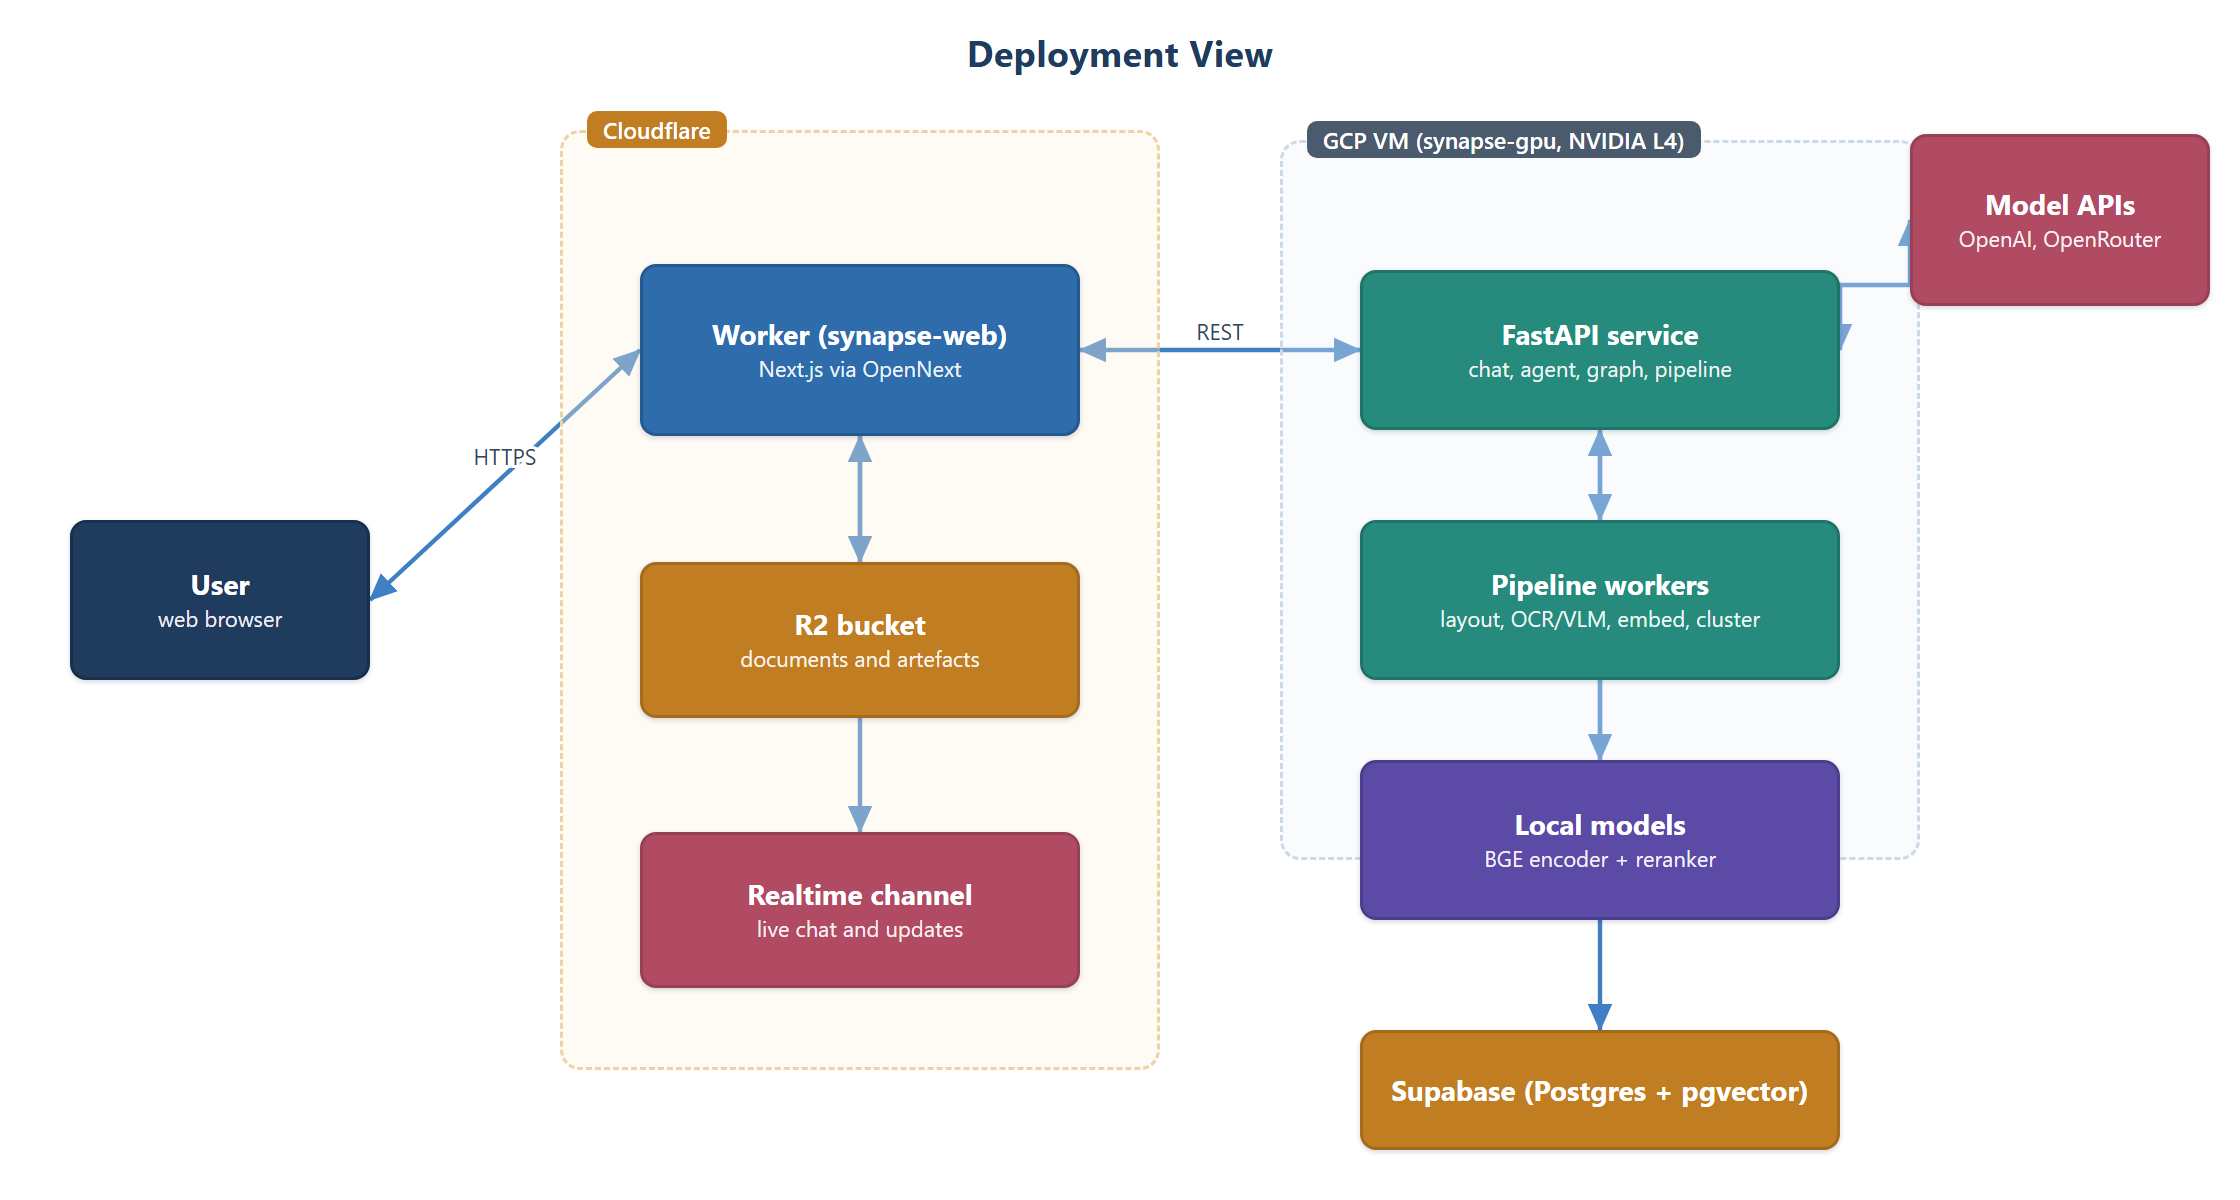
\includegraphics[width=\textwidth]{fig_deployment.png}
  \caption{Deployment view. The application and its object store run on Cloudflare
  at the edge, while document processing, retrieval and the local models run on a
  single GPU virtual machine. The managed database provides vector search, and the
  external model services are called over the network. The split keeps the
  interface responsive and the processing in one place.}
  \label{fig:deployment}
\end{figure}

\section{Summary}

This chapter presented the architecture of Synapse and the principles of
grounding, separation of concerns, resumable processing and tenant isolation that
shaped it. It described the design of the grounded chat, which grades evidence
before answering and abstains when it is insufficient; the agent, which builds
faithful artefacts by binding data in code; and the knowledge graph, which keeps
provenance back to the source. It then presented the data model and the deployment
arrangement. The next chapter explains how this design was implemented.

\chapter{Implementation}
\label{ch:implementation}

\section{Introduction}

This chapter explains how the design of Chapter~4 was built. It describes the
technology stack, the ingestion pipeline that processes documents, and the
implementation of the retrieval, agent and knowledge-graph subsystems. It also
covers how data, storage and security were realised. The aim is to show the main
modules and how they fit together, rather than to reproduce the code in full.

\section{Technology Stack}

The platform was built from established, well-supported technologies, chosen so
that the team could concentrate on the design rather than on infrastructure.
Table~\ref{tab:stack} summarises the stack and the role of each part.

\begin{table}[H]
  \centering
  \caption{The technology stack and the role of each component. The user-facing
  application runs at the edge on Cloudflare, the processing and reasoning run on a
  GPU server, and the data lives in a managed database and object store, with
  language and vision models reached over the network.}
  \label{tab:stack}
  \small
  \begin{tabularx}{\textwidth}{@{}p{0.28\textwidth}X@{}}
    \toprule
    \textbf{Layer} & \textbf{Technology and role} \\
    \midrule
    Web application      & Next.js and React, deployed to a Cloudflare Worker through OpenNext, providing the user interface at the edge. \\
    Backend service      & FastAPI in Python, running on a GPU virtual machine, exposing the chat, agent, graph and pipeline interfaces. \\
    Database             & Supabase (PostgreSQL) with the pgvector extension for vector search and full-text search for keywords. \\
    Object storage       & Cloudflare R2 for the original files, the processed text, and the generated artefacts. \\
    Local models         & The BGE encoder for embeddings and a cross-encoder reranker, run on the server's GPU. \\
    Hosted models        & OpenAI and OpenRouter, providing the language models and the Qwen2.5-VL vision-language model. \\
    Document analysis    & DocLayout-YOLO for page layout and an optical character recognition toolkit for scanned text. \\
    Real-time            & Supabase Realtime, which delivers live chat and processing updates to the browser. \\
    \bottomrule
  \end{tabularx}
\end{table}

\section{The Ingestion Pipeline}

The ingestion pipeline turns a connected source into a searchable library. It is
implemented as a sequence of queue-driven stages, shown in
Figure~\ref{fig:pipeline}, each carried out by its own worker. A stage runs in
batches and only begins once the previous stage has completed for a document,
which makes the whole pipeline resumable: if a stage fails, it can be retried
without redoing the work that came before it.

\begin{figure}[H]
  \centering
  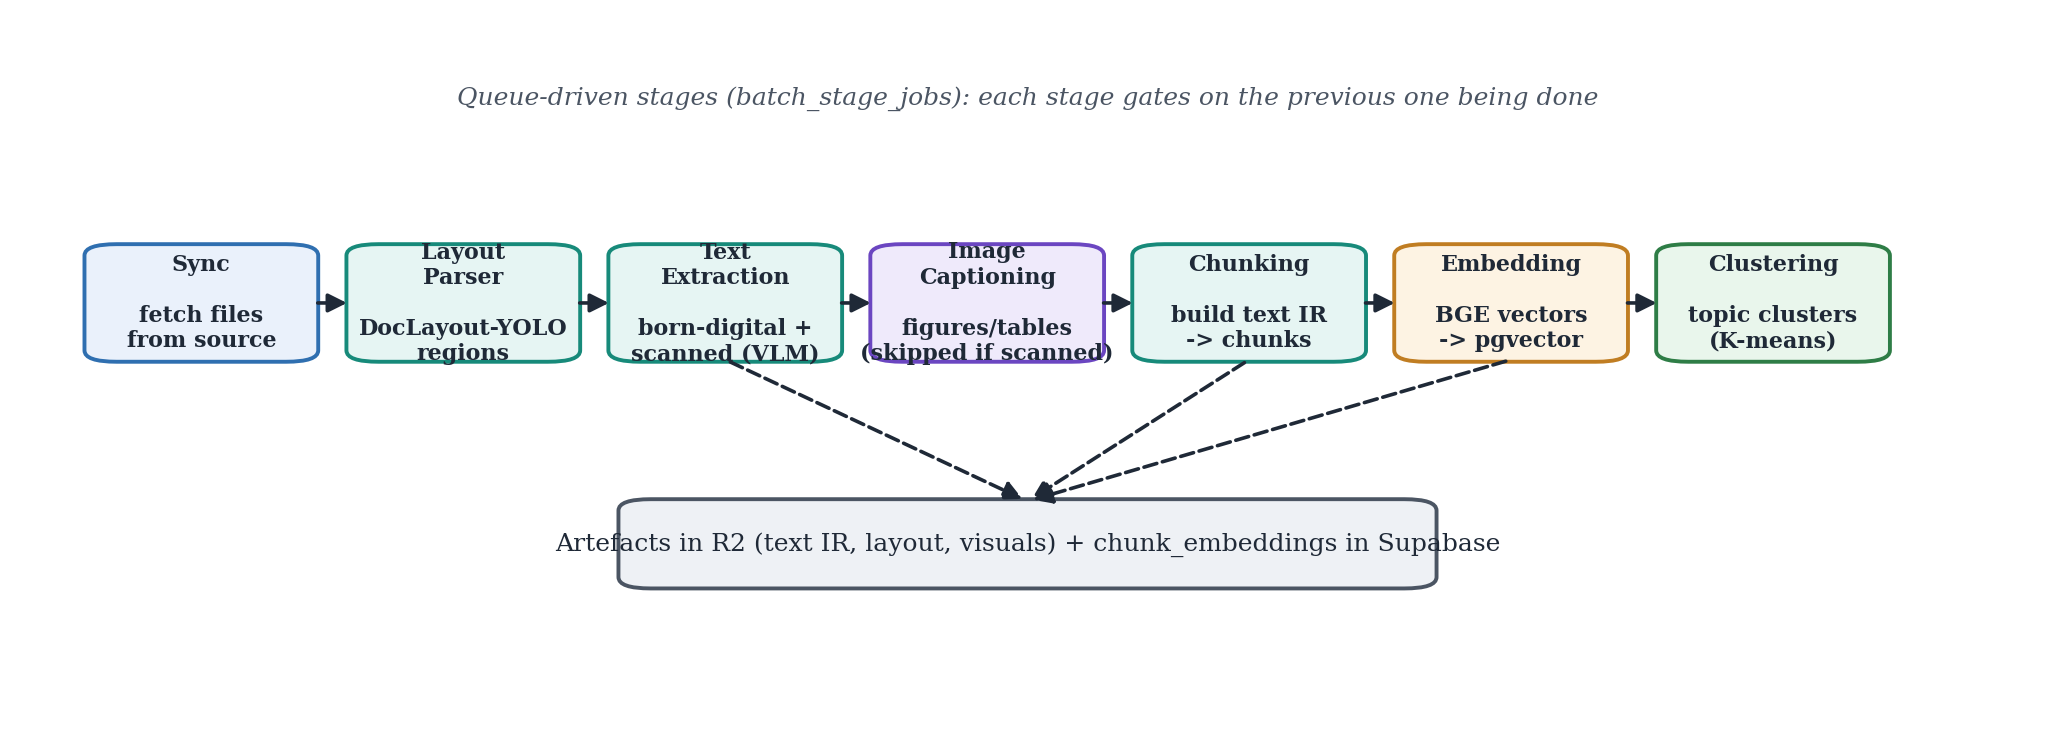
\includegraphics[width=\textwidth]{fig_pipeline.png}
  \caption{The implemented ingestion pipeline. Each stage is a separate worker
  that runs in batches and waits for the previous stage to finish, so processing
  is resumable and a failure in one document or stage does not lose the rest. The
  text and visuals are stored as artefacts, and the chunk embeddings are written
  to the vector database for retrieval.}
  \label{fig:pipeline}
\end{figure}

The stages map onto the worker modules of the backend. A sync worker fetches the
files from the connected source. A layout worker detects the regions of each page
using DocLayout-YOLO. An extraction worker reads the text, taking born-digital
text directly and reading scanned pages with the vision-language model through a
dedicated client. A captioning worker describes figures and tables. A chunking
worker splits the text into passages, an embedding worker encodes each passage
with the BGE model and writes it to the vector database, and a clustering worker
groups the passages into topics for coverage. A batch creator schedules the work
and a watchdog recovers stages that stall, so that large libraries are processed
steadily and reliably.

\section{Retrieval and the Grounded Chat}

The grounded chat is implemented around a runtime that carries out the
grade-then-answer flow from Chapter~4. When a question arrives, the chat interface
hands it to the runtime, which embeds the question, retrieves passages by vector
and by keyword, fuses the two ranked lists with reciprocal rank fusion, and
re-ranks the result with the cross-encoder. The agents that plan the retrieval,
grade the evidence and compose the answer are kept as separate, small steps, which
made each one easy to test and adjust. A retriever worker and a queue allow the
heavier retrieval work to run without blocking the interface.

The decision to answer or abstain is made explicitly after the evidence has been
graded. Listing~\ref{lst:abstain} shows this decision in simplified form: the
system only composes an answer when the graded evidence clears a confidence
threshold, and otherwise returns an honest abstention. The actual implementation
adds citation tracking and the option to refine the query and retrieve again
before abstaining.

\begin{lstlisting}[language=Python,caption={Simplified grade-then-answer decision in the chat runtime.},label={lst:abstain}]
graded = grade_evidence(question, reranked_passages)

if graded.is_sufficient and graded.confidence >= ABSTAIN_THRESHOLD:
    answer = compose_answer(question, graded.passages)
    return answer.with_citations(graded.passages)
else:
    return abstain("The selected library does not support an answer.")
\end{lstlisting}

\section{The Agent}

The agent is implemented as a small set of steps coordinated by an agent
interface. A language-model client targets a capable hosted model and returns
structured results, which are validated before use. The planning, data-extraction
and specification steps are separate functions, mirroring the design in
Chapter~4. Structured files are read exactly by a data module that preserves the
native cell types of a spreadsheet, while unstructured needs are met by reuse of
the retrieval stack. A specification module validates a chart or diagram and binds
the data values to it in code, and separate modules handle the rendering of
documents and images. Keeping the model's role to describing artefacts, and
binding data outside the model, is what makes the figures faithful.

\section{The Knowledge Graph}

The knowledge graph is implemented in four parts that follow its construction
flow. An extraction module prompts a language model to list the entities and
relationships in each chunk. A resolution module merges entities that refer to the
same thing under different names. A build module assembles the nodes and edges and
scores their weights, and an interface module serves the graph to the web
application, where it is drawn as an interactive diagram. Throughout, each node
and edge records the chunk it came from, so the graph remains connected to its
evidence.

\section{Data, Storage and Security}

The data described in Chapter~4 is stored in PostgreSQL through Supabase, with the
pgvector extension providing the vector search used by retrieval and a full-text
index providing the keyword search. The original files, the processed text and the
generated artefacts are kept in Cloudflare R2. Tenant isolation is enforced by
row-level security: every table that holds tenant data carries an organisation
identifier, and database policies ensure that a member can read only the rows that
belong to their organisation. This places the privacy guarantee at the database,
where it cannot be bypassed by a mistake in the application. Live updates, such as
new chat messages and changes in processing status, are delivered to the browser
through Supabase Realtime.

\section{Summary}

This chapter described the implementation of the platform. It set out the
technology stack, explained the queue-driven ingestion pipeline and its worker
modules, and described how the grounded chat, the agent and the knowledge graph
were built from small, separate steps that follow their designs. It also explained
how the data model, storage and the row-level security that guarantees tenant
isolation were realised. The next chapter presents the finished product through
the web application.

\chapter{The Product}
\label{ch:product}

\section{Introduction}

This chapter presents the finished platform as a user experiences it. It walks
through the web application feature by feature, using screenshots of the running
system: connecting and processing libraries, asking grounded questions,
collaborating as a team, generating visuals and documents with the agent, saving
the resulting artefacts, and exploring the knowledge graph. Together these views
show that the design and implementation of the previous chapters come together
into a single, usable product.

\section{Libraries and Processing}

The starting point is the libraries view, shown in Figure~\ref{fig:ui-libraries}.
A user connects a source and creates a library, and the platform processes its
documents through the pipeline described in Chapter~5. Each library shows its
processing state and a progress bar, so the user can see at a glance when a
collection is ready to be used. The figure shows several processed libraries,
including collections of research papers, spreadsheets and source code, each
marked as complete.

\begin{figure}[H]
  \centering
  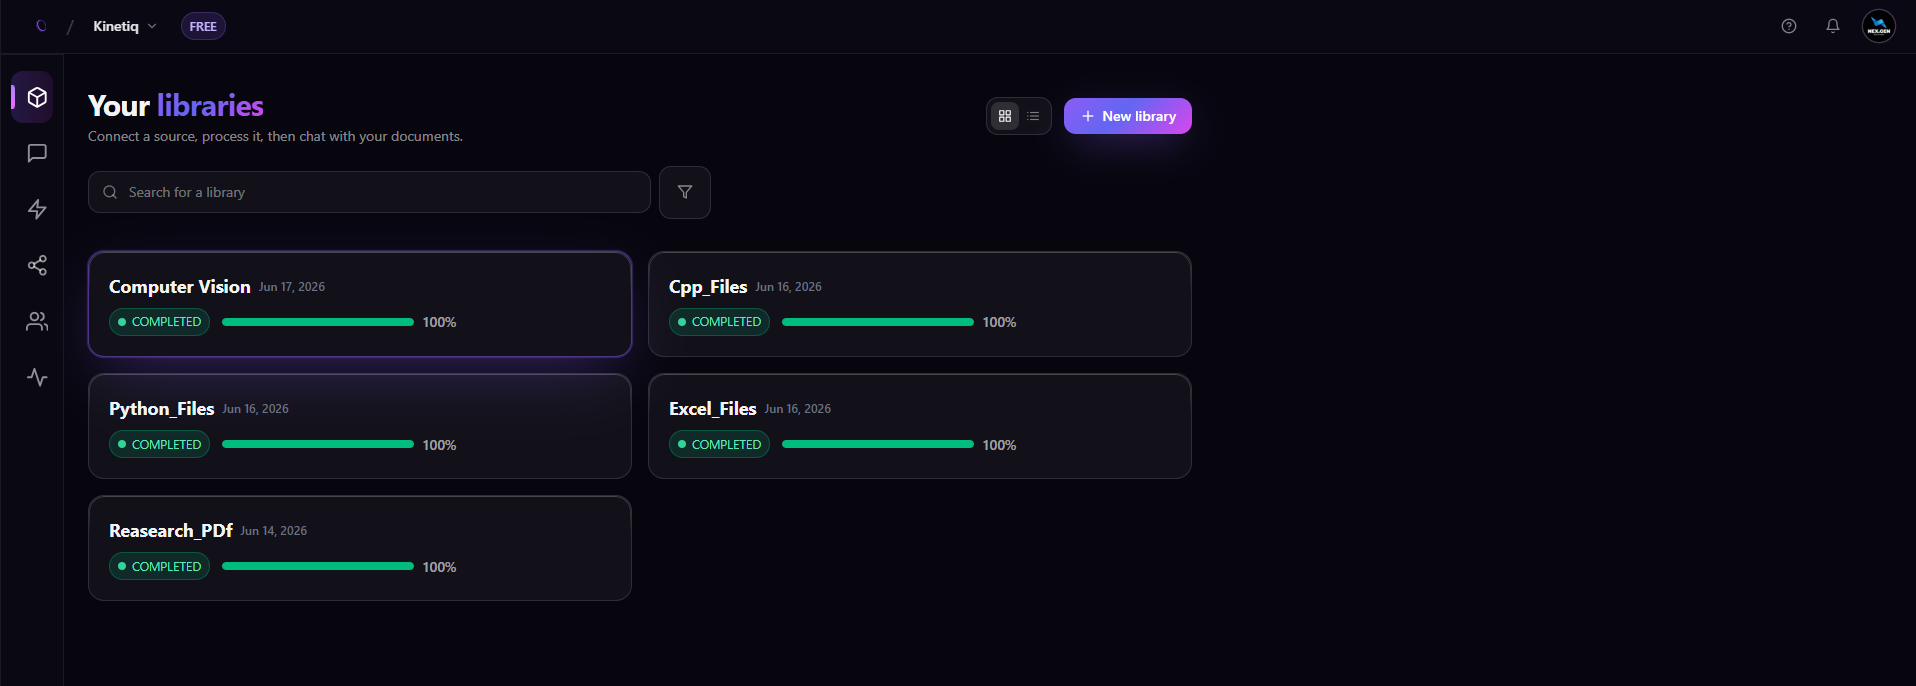
\includegraphics[width=\textwidth]{Preprocess_Libraries.png}
  \caption{The libraries view. A user creates a library from a connected source,
  and the platform processes its documents in the background. Each card shows the
  library's status and progress, here several completed collections of papers,
  spreadsheets and code. From this view the user moves on to questioning,
  visualising or mapping a library.}
  \label{fig:ui-libraries}
\end{figure}

\section{Grounded Chat}

The chat view, shown in Figure~\ref{fig:ui-chat}, is where a user asks questions
of a library. The answer is written in plain language and is followed by the
sources it relied on, so that each claim can be checked against the document it
came from. In the figure the user asks which student has the highest average, and
the platform answers with the specific value and lists the source it used. This is
the grounded, citing behaviour designed in Chapter~4 in action.

\begin{figure}[H]
  \centering
  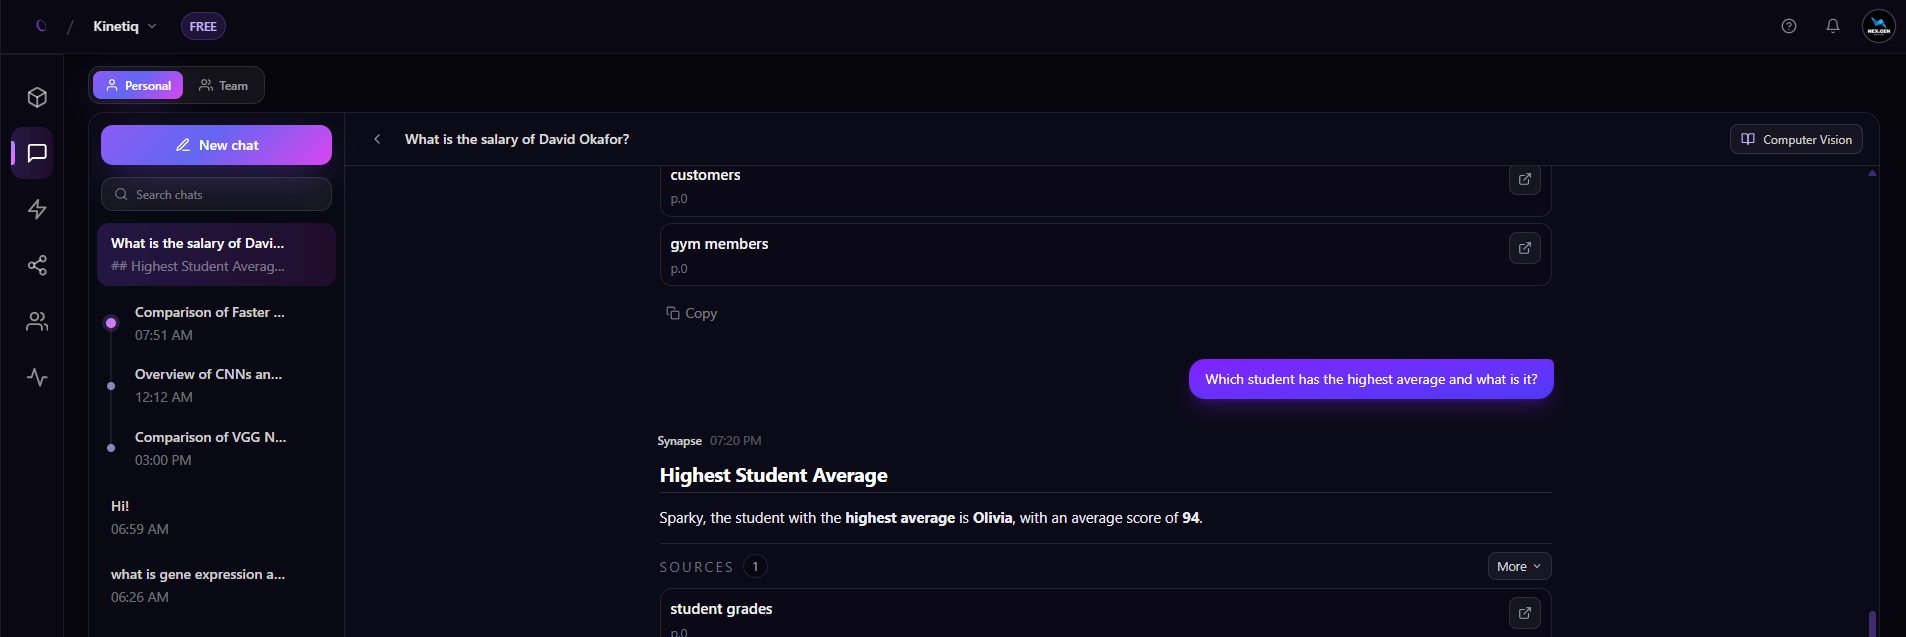
\includegraphics[width=\textwidth]{QA_with_doc.png}
  \caption{The grounded chat. The user asks a question and the platform answers
  from the selected library, listing the source passages beneath the answer. The
  reply gives a specific, grounded result rather than a vague summary, and the
  cited source lets the user verify it. When the library cannot support an answer,
  the platform says so instead of guessing.}
  \label{fig:ui-chat}
\end{figure}

\section{Team Collaboration}

The same chat can be used by a team. Figure~\ref{fig:ui-team} shows the team view,
where members of an organisation share libraries and a conversation. Messages are
attributed to the member who sent them, and the assistant's grounded replies,
including tables where they help, are visible to everyone in real time. This turns
the platform from a personal tool into a shared workspace over a common set of
documents.

\begin{figure}[H]
  \centering
  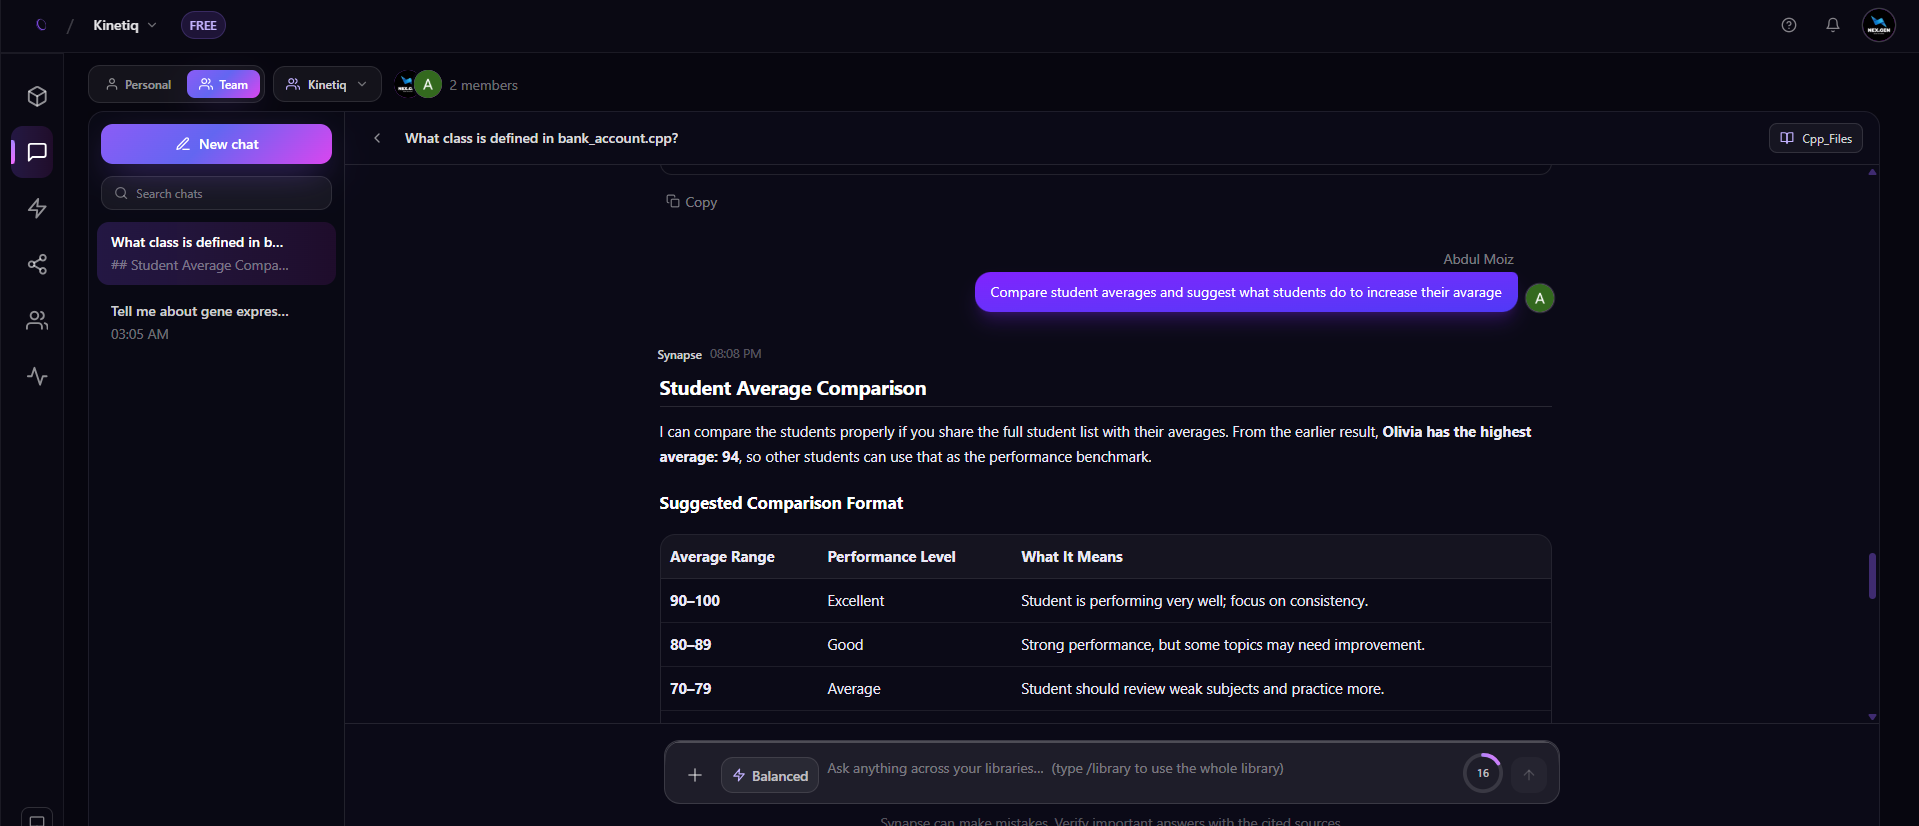
\includegraphics[width=\textwidth]{Team_Chats.png}
  \caption{The team chat. Members of an organisation share libraries and a
  conversation, with each message attributed to its sender and the grounded
  replies visible to all in real time. Here a member asks for a comparison and the
  assistant responds with a structured answer. The realtime channel keeps every
  member's view in step.}
  \label{fig:ui-team}
\end{figure}

\section{Agent: Generating Visuals}

The agent view, shown in Figure~\ref{fig:ui-visuals}, turns a library or an
attached file into visuals. The user chooses the kinds of visual to allow, such as
bar, line or pie charts, and states a goal in plain language. The agent produces
the charts together with a short written explanation, including the assumptions it
made and recommendations for a clearer presentation, and each chart can be
downloaded as an image. The figure shows a grouped bar chart and a line chart
generated from a spreadsheet, with the numbers taken directly from the source.

\begin{figure}[H]
  \centering
  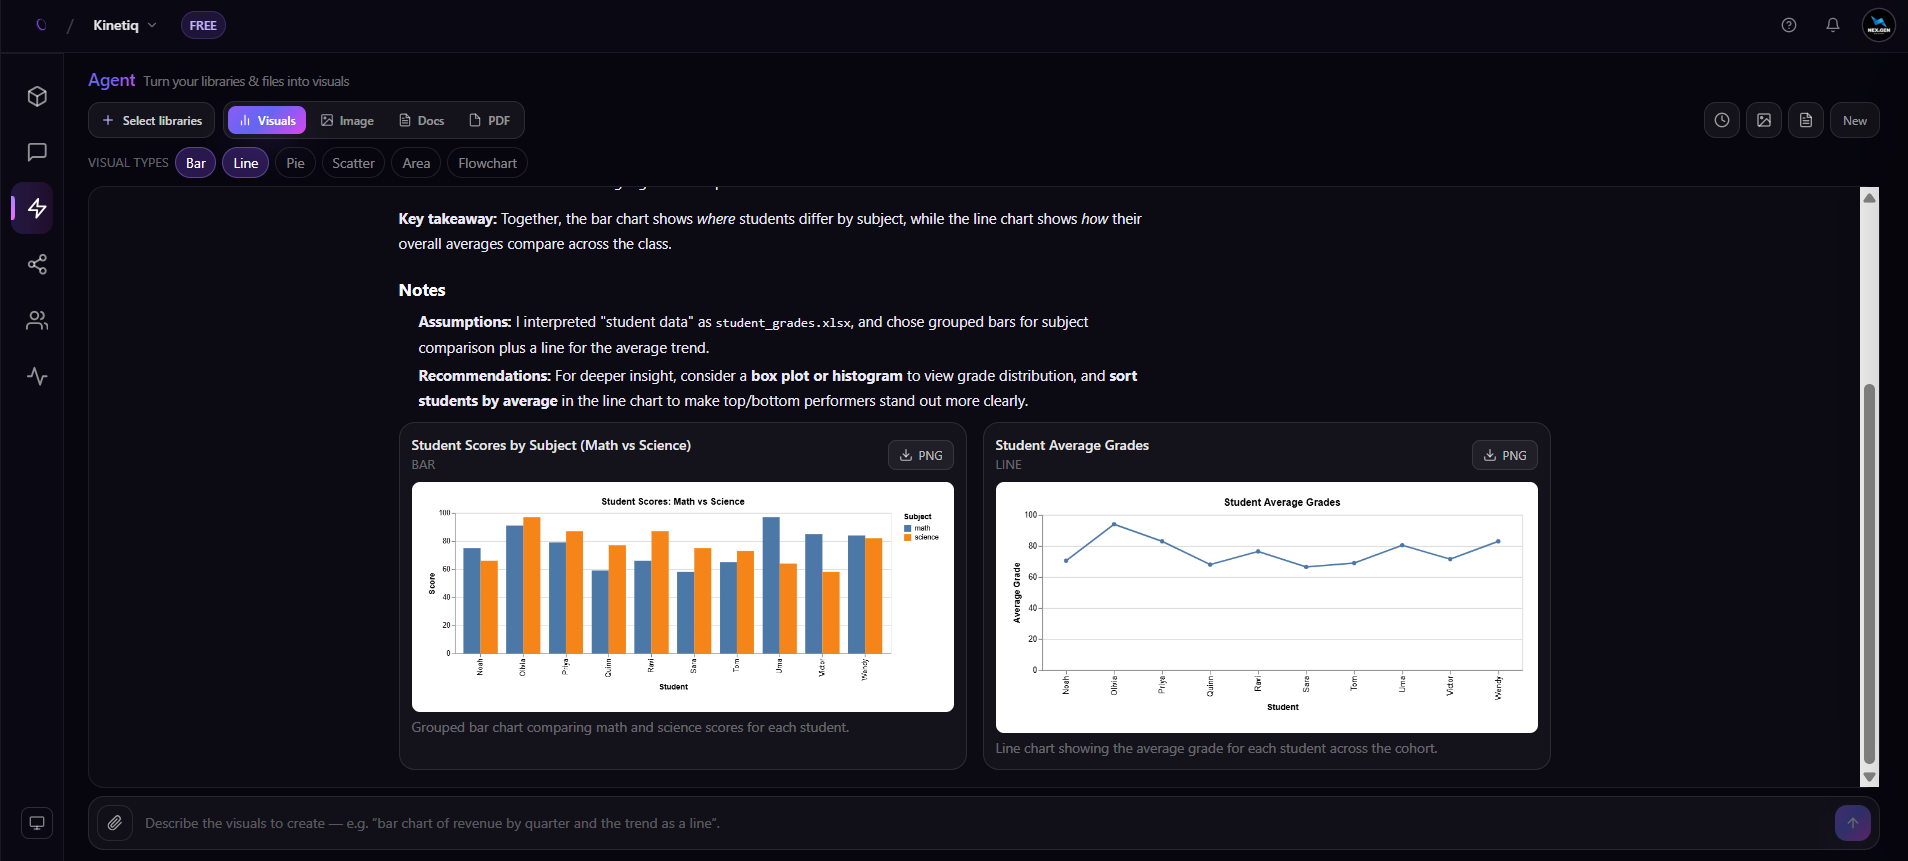
\includegraphics[width=\textwidth]{Generate_Visuals.png}
  \caption{The agent generating visuals. From a spreadsheet and a plain-language
  goal, the agent produces a grouped bar chart and a line chart, each downloadable
  as an image, alongside a written explanation with its assumptions and
  recommendations. Because the values are bound from the source file, the charts
  are faithful to the underlying data.}
  \label{fig:ui-visuals}
\end{figure}

\section{Agent: Generating Documents}

The agent also drafts written documents, as shown in Figure~\ref{fig:ui-docs}.
From a request and the connected sources it produces a document, offered both as a
readable draft and as a downloadable file in Markdown or PDF form. In the figure
the agent has drafted several documents from the user's computer-vision sources,
each available to read or download. This lets a user turn a library into a report
or a structured summary without leaving the platform.

\begin{figure}[H]
  \centering
  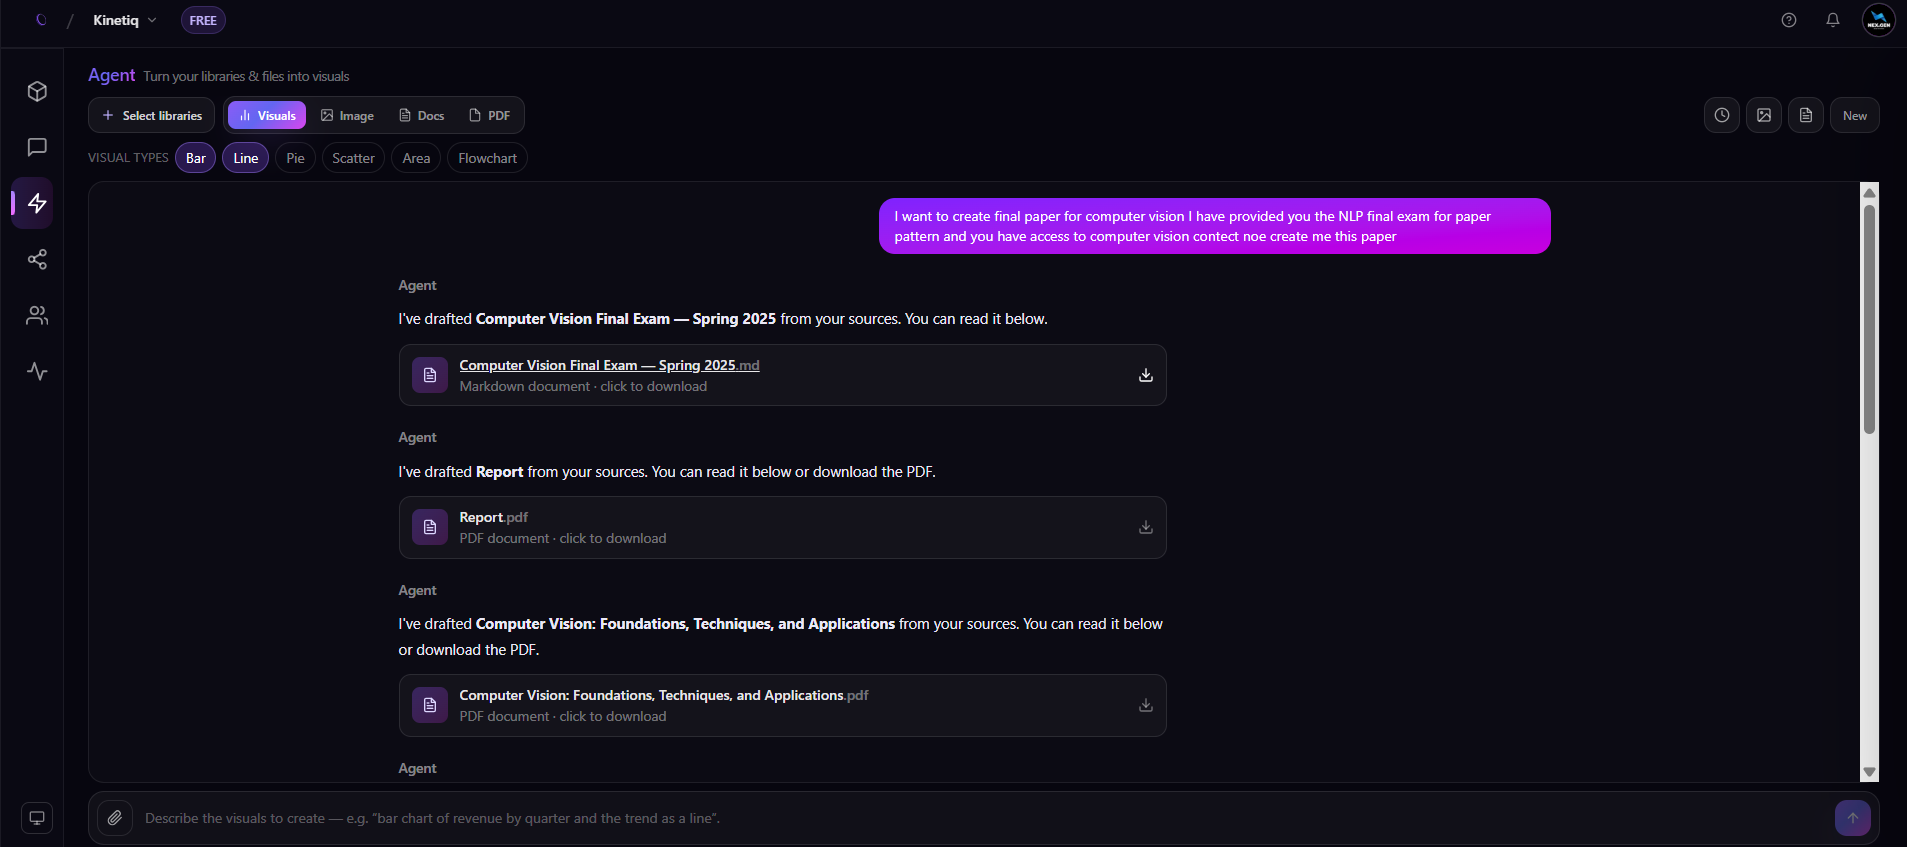
\includegraphics[width=\textwidth]{Generate_doc.png}
  \caption{The agent generating documents. From the connected sources the agent
  drafts written documents and offers them as downloadable Markdown or PDF files.
  Several drafts produced from the user's sources are shown, each ready to read or
  download. The documents are written from the library, so they reflect the user's
  own material.}
  \label{fig:ui-docs}
\end{figure}

\section{Saved Artefacts}

The artefacts the agent produces are kept for later use. Figure~\ref{fig:ui-saved}
shows the saved-visuals panel, which collects the charts a user has generated, each
with its title, a short description and a download option. This means that work
done with the agent is not lost when the conversation ends, and a user can return
to a chart and reuse it.

\begin{figure}[H]
  \centering
  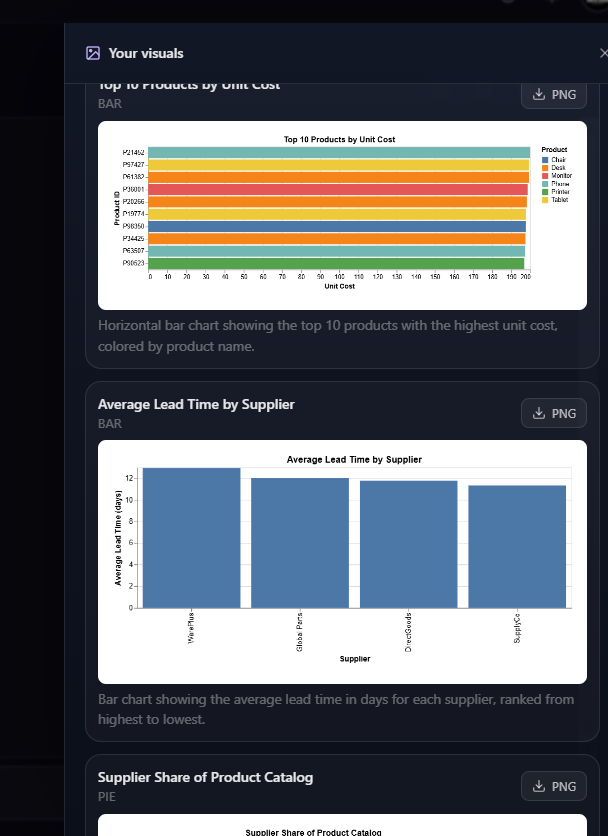
\includegraphics[width=0.52\textwidth]{Save_Visual_docs.png}
  \caption{The saved-artefacts panel. Charts generated by the agent are collected
  here with their titles and descriptions, each downloadable as an image. Keeping
  the artefacts means a user can return to earlier work and reuse it rather than
  regenerate it. The panel gathers visuals produced across different requests in
  one place.}
  \label{fig:ui-saved}
\end{figure}

\section{Knowledge Graph}

Finally, the platform can map a library as a knowledge graph. Building the graph
runs as a background task with clear progress, shown in
Figure~\ref{fig:ui-kg-build}, as the system reads the documents and extracts
entities. The finished graph, shown in Figure~\ref{fig:ui-kg-view}, draws the
entities as nodes coloured by type, such as concept, method, system and product,
and lets the user explore how they connect across the library. The user can
rebuild the graph or switch to a different library.

\begin{figure}[H]
  \centering
  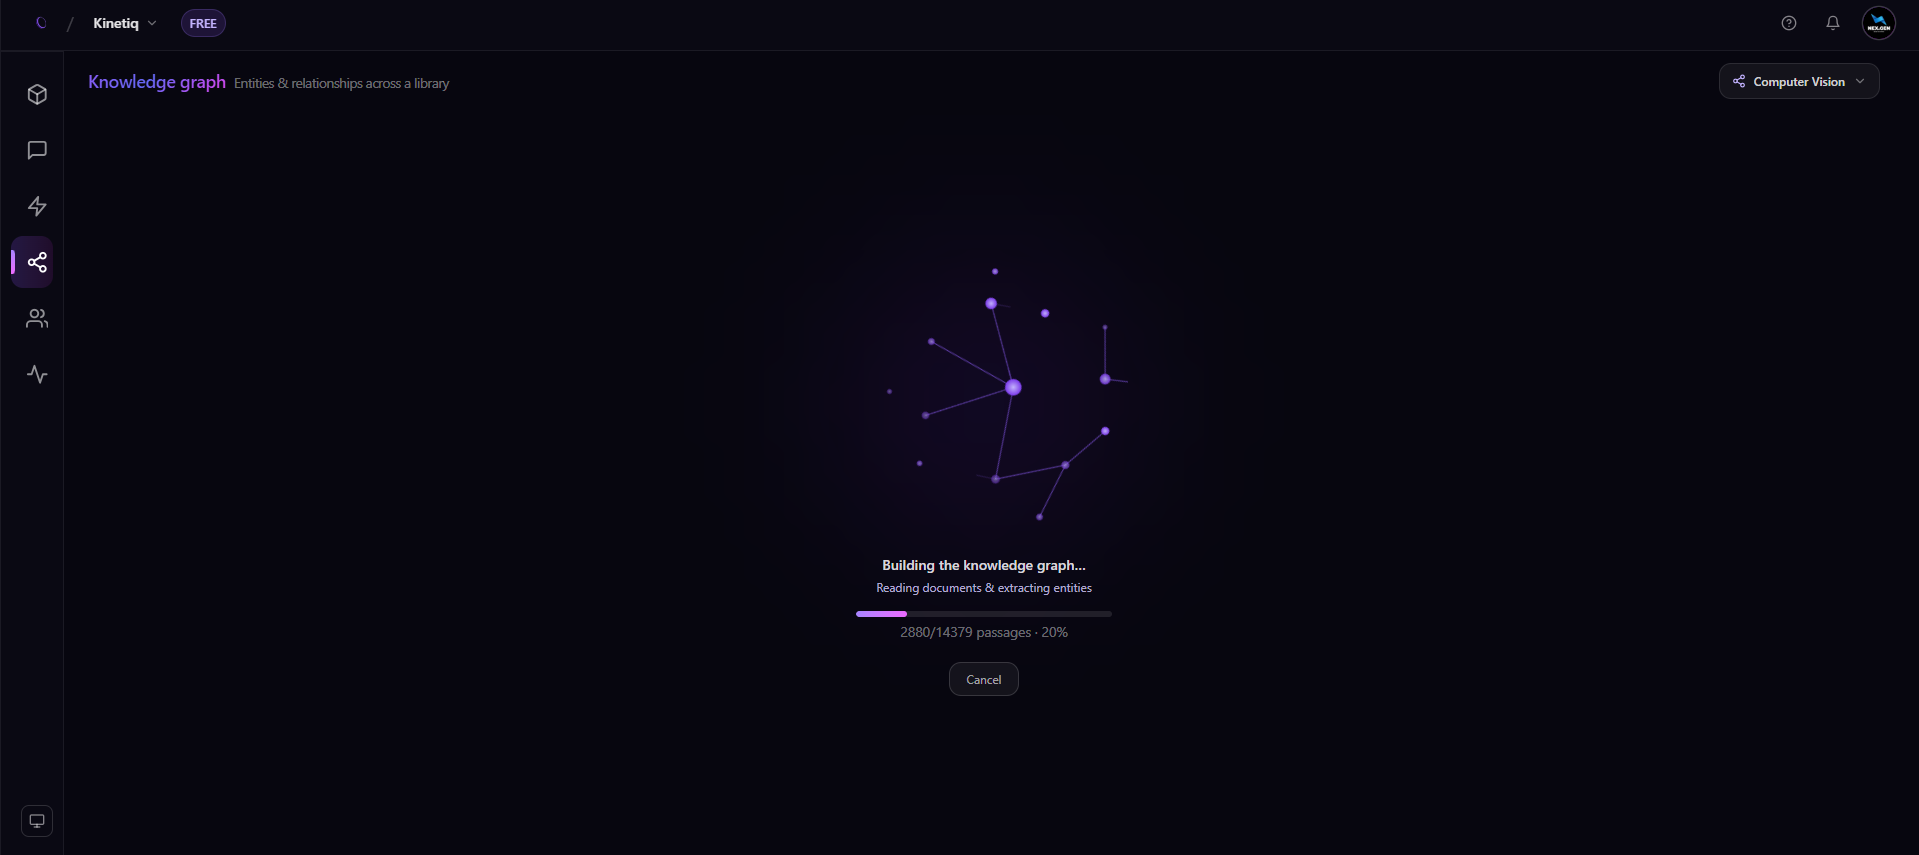
\includegraphics[width=\textwidth]{Knowledge_graph_generation.png}
  \caption{Building the knowledge graph. The platform reads the documents of a
  library and extracts entities and relationships as a background task, showing the
  number of passages processed and the overall progress. The user can cancel the
  build if needed. This is the construction flow from Chapter~4 as the user sees
  it.}
  \label{fig:ui-kg-build}
\end{figure}

\begin{figure}[H]
  \centering
  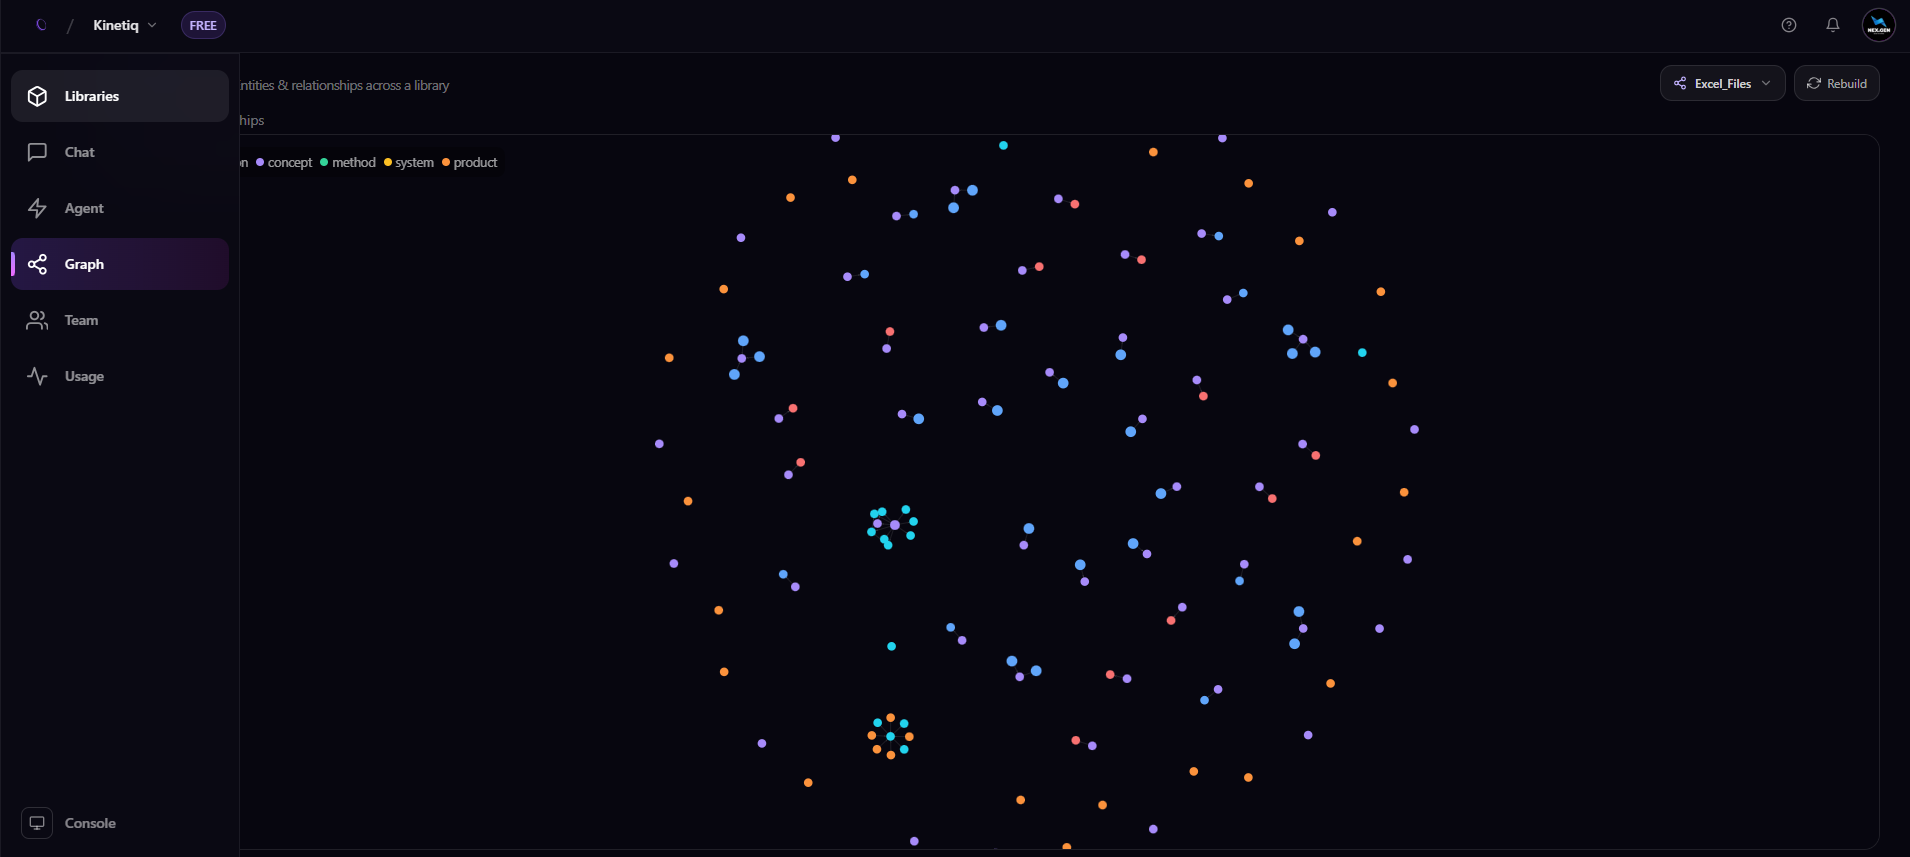
\includegraphics[width=\textwidth]{Knowledge_graph_representaiton.png}
  \caption{The interactive knowledge graph. The entities of a library are drawn as
  nodes coloured by type, such as concept, method, system and product, and the user
  can explore how they connect. A library selector and a rebuild control sit at the
  top. The graph turns a flat collection of documents into a structure the user can
  navigate.}
  \label{fig:ui-kg-view}
\end{figure}

\section{Summary}

This chapter presented the finished product through the web application. It showed
how a user connects and processes libraries, asks grounded questions and sees the
sources behind each answer, collaborates with a team in real time, generates
faithful visuals and written documents with the agent, keeps the resulting
artefacts, and maps a library as an interactive knowledge graph. These views
demonstrate that the platform delivers, in a single usable interface, the
capabilities set out at the start of the thesis. The next chapter evaluates how
well it performs.

\chapter{Testing and Evaluation}
\label{ch:evaluation}

\section{Introduction}

This chapter evaluates how well the platform meets its goals. It describes the
evaluation method, then reports the results for retrieval accuracy, answer quality
and honesty, citation quality, understanding of structured documents, and
efficiency. It also summarises the functional testing of the agent and the
knowledge graph. The aim throughout is to judge not only whether the answers are
correct, but also whether the system is honest about what it does not know.

\section{Evaluation Method}

The platform was evaluated in three complementary ways. First, the grounded chat
was assessed on the DOUBLE-BENCH document benchmark \cite{shen2025doublebench},
which poses questions over realistic, multimodal documents and requires one or
several hops of reasoning to answer. This benchmark was chosen because it tests
exactly the setting Synapse targets: retrieval and answering over mixed documents,
including scanned and visually rich pages. Retrieval was measured by whether the
correct source document appeared among the retrieved results, and answers were
graded for correctness.

Second, three purpose-built datasets were created to test the understanding of
structured documents: a set of spreadsheets, a set of Python source files and a
set of C++ source files, each paired with questions whose answers are known. These
let the system's answers be checked exactly against the source, which is harder to
do with free-form prose.

Third, the agent and the knowledge graph were tested functionally, by running
representative tasks end to end and checking that the artefacts and graphs produced
were correct and usable. Because grading free-form answers by hand does not scale,
answer correctness on the benchmark was judged automatically by two independent
language-model judges \cite{zheng2023judge}, and their agreement was recorded so
that the reliability of the grading could itself be assessed.

\section{Retrieval Accuracy}

Retrieval is the foundation of every answer, so it was measured first.
Figure~\ref{fig:eval-retrieval} reports the document-level hit rate, that is, how
often the correct source document was among those retrieved. Retrieval was strong
overall and was essentially perfect on questions that depend on a single document.
It fell on the hardest questions, those that require evidence to be combined across
three documents, which is the expected pattern: the more pieces of evidence a
question needs, the more chances there are to miss one. Retrieval was slightly
lower on scanned documents than on born-digital ones, reflecting the additional
difficulty of reading a scanned page, but the gap was small.

\begin{figure}[H]
  \centering
  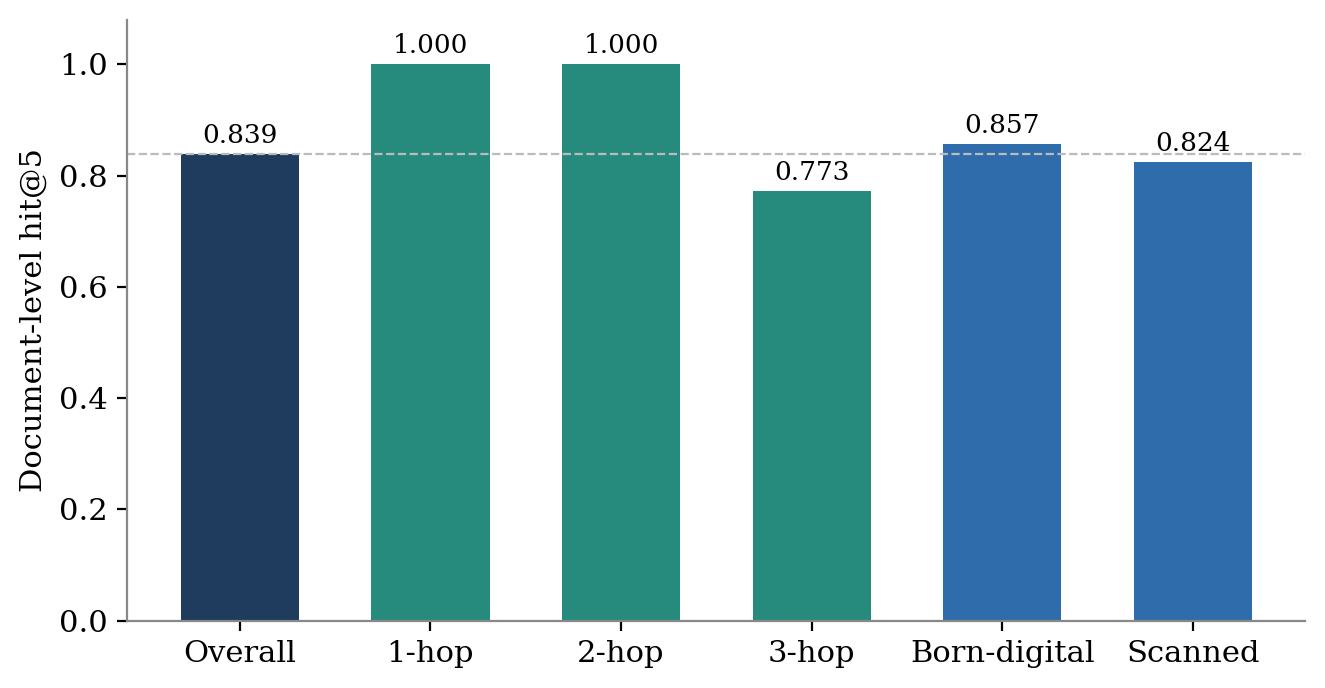
\includegraphics[width=0.86\textwidth]{fig_eval_retrieval.png}
  \caption{Document-level retrieval accuracy (hit@5). Retrieval is near-perfect on
  single-document questions and remains strong overall, falling only on the hardest
  questions that require evidence from three documents at once. The small gap
  between born-digital and scanned documents shows that the pipeline reads scanned
  pages effectively. The dashed line marks the overall rate.}
  \label{fig:eval-retrieval}
\end{figure}

\section{Answer Quality and Honesty}

Answer correctness was graded by two independent judges, whose results are shown in
Figure~\ref{fig:eval-answers}. Both judges found that a substantial share of
answers were fully correct, with a further portion partially correct, and the two
judges agreed on three quarters of their verdicts, which gives reasonable
confidence in the grading. The judges differed in strictness, as automatic judges
often do, but they agreed on the overall picture: the system answers a large
fraction of difficult, multi-hop questions correctly while still leaving room to
improve on the hardest cases.

\begin{figure}[H]
  \centering
  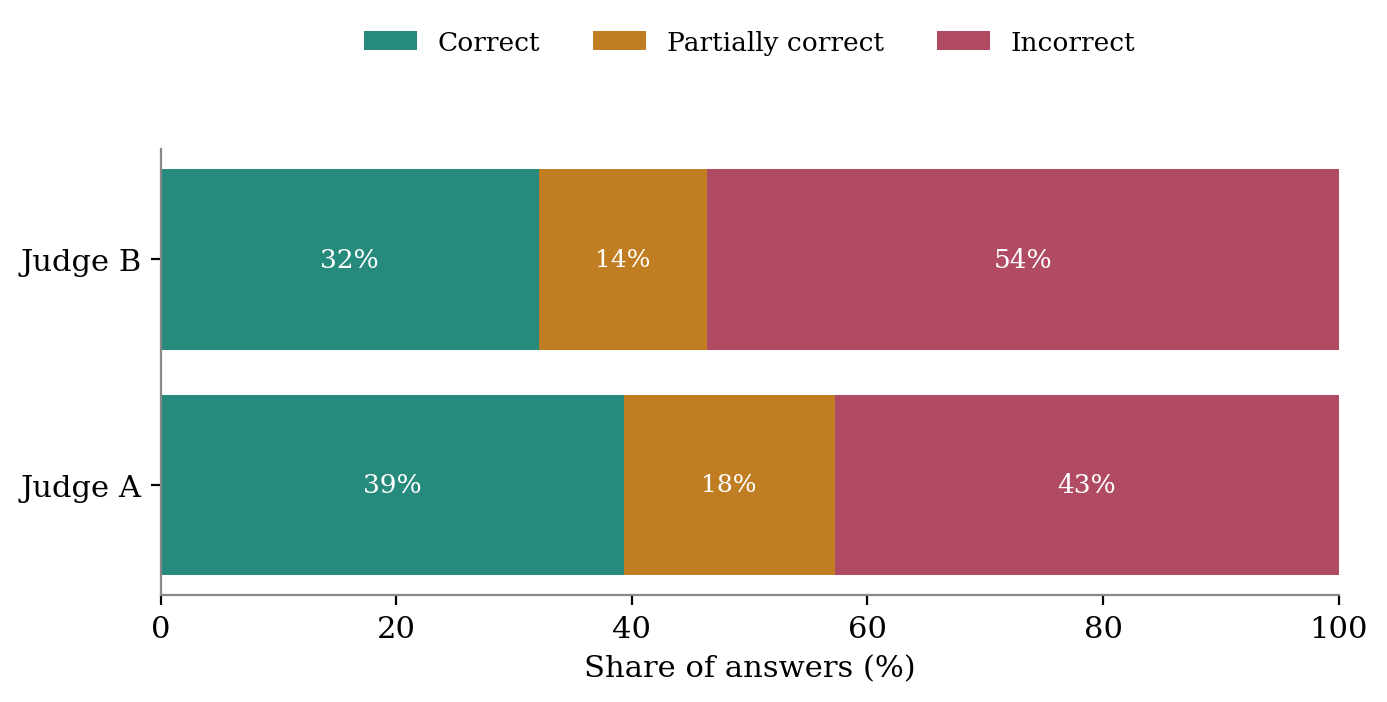
\includegraphics[width=0.86\textwidth]{fig_eval_answers.png}
  \caption{Answer correctness as graded by two independent judges. Each bar shows
  the share of answers judged correct, partially correct and incorrect. The two
  judges agreed on about three quarters of their verdicts; they differ in
  strictness but agree that the system answers a large share of difficult,
  multi-hop questions correctly.}
  \label{fig:eval-answers}
\end{figure}

Correctness alone does not capture honesty. A system that answers every question,
right or wrong, is less trustworthy than one that declines when it should. The
overconfidence rate, the share of answers that were given confidently but were
wrong, was low at $0.148$, and applying the abstention threshold designed in
Chapter~4 roughly halved it to $0.074$. In other words, allowing the system to
abstain removed about half of its confident mistakes, which is exactly the
behaviour the design aimed for.

\section{Citation Quality}

Because every claim is meant to carry a citation, the citations themselves were
measured. Table~\ref{tab:citation} reports their precision and recall. Precision
was perfect, meaning that every passage the system cited was genuinely relevant to
the claim it supported, and recall was high, meaning that almost every claim that
needed a citation received one. Reliable citations are what allow a user to trust,
and to check, the answers.

\begin{table}[H]
  \centering
  \caption{Citation quality. Precision measures whether cited passages are
  genuinely relevant; recall measures whether claims that need a citation receive
  one. Perfect precision and high recall mean the citations can be relied upon to
  verify an answer.}
  \label{tab:citation}
  \small
  \begin{tabularx}{0.7\textwidth}{@{}Xcc@{}}
    \toprule
    \textbf{Metric} & \textbf{Precision} & \textbf{Recall} \\
    \midrule
    Citation quality & $1.000$ & $0.963$ \\
    \bottomrule
  \end{tabularx}
\end{table}

\section{Understanding Structured Documents}

The three purpose-built datasets tested whether the system can answer exactly from
structured documents. Figure~\ref{fig:eval-datasets} reports the share of questions
whose answer matched the known value. Accuracy was high on all three: the system
read spreadsheets, Python and C++ files and answered most questions exactly. The
few failures were concentrated on questions that require aggregating across many
rows or that depend on a passage the retrieval step did not surface, which points
to where the most useful improvements lie.

\begin{figure}[H]
  \centering
  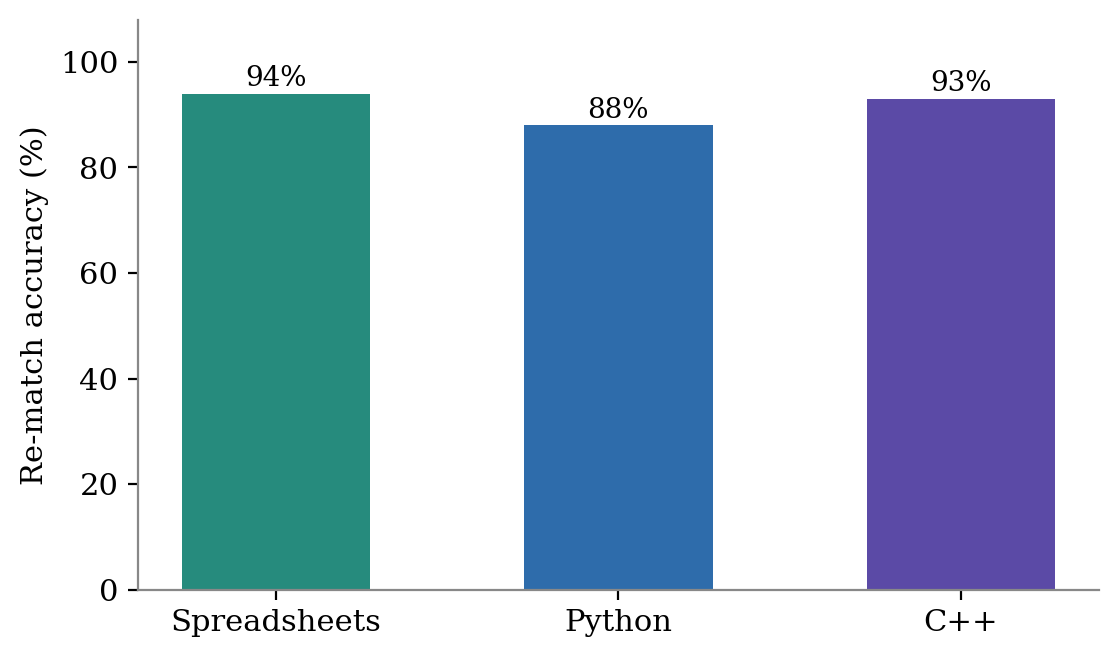
\includegraphics[width=0.66\textwidth]{fig_eval_datasets.png}
  \caption{Exact-match accuracy on the purpose-built structured datasets. The
  system answered most questions about spreadsheets, Python files and C++ files
  exactly against the known value. The remaining failures were mainly questions
  needing aggregation across many rows or a passage that was not retrieved, which
  indicates the clearest avenues for improvement.}
  \label{fig:eval-datasets}
\end{figure}

\section{Efficiency}

Response time matters for a usable product, so the latency of the main operations
was measured. Table~\ref{tab:efficiency} reports representative figures. Retrieval
returns its first evidence in about two seconds, so the interface feels responsive.
A full, deep answer that reasons over several passages takes longer, with a typical
time of around half a minute and a long tail on the most demanding questions, which
is the expected cost of the careful, multi-step reasoning that makes the answers
reliable.

\begin{table}[H]
  \centering
  \caption{Representative response times. Retrieval is fast enough for the
  interface to feel immediate, while a full multi-step answer takes longer, with a
  long tail on the most demanding questions. The extra time buys the careful
  retrieval and grading that keep the answers grounded.}
  \label{tab:efficiency}
  \small
  \begin{tabularx}{0.86\textwidth}{@{}Xccc@{}}
    \toprule
    \textbf{Operation} & \textbf{Median} & \textbf{90th pct.} & \textbf{99th pct.} \\
    \midrule
    Evidence retrieval        & $2.0$\,s  & --        & --        \\
    Full multi-step answer    & $32$\,s   & $83$\,s   & $143$\,s  \\
    \bottomrule
  \end{tabularx}
\end{table}

\section{Functional Testing}

The agent and the knowledge graph were tested by running representative tasks from
end to end. Table~\ref{tab:functional} summarises the checks and their outcomes.
The agent produced correct charts and documents, asked for clarification only when
a request was genuinely ambiguous, and kept chart values faithful to the source.
The knowledge graph built successfully from a processed library, drew the entities
and their relationships, and kept each element linked back to its source. All of
the checks passed.

\begin{table}[H]
  \centering
  \caption{Functional testing of the agent and knowledge graph. Each
  representative task was run end to end and checked against the expected
  behaviour. All checks passed, confirming that the artefact and graph features
  behave as designed.}
  \label{tab:functional}
  \small
  \begin{tabularx}{\textwidth}{@{}p{0.07\textwidth}Xc@{}}
    \toprule
    \textbf{No.} & \textbf{Check} & \textbf{Result} \\
    \midrule
    T-1 & A chart request produces a chart whose values match the source file. & Pass \\
    T-2 & A document request produces a readable, downloadable document. & Pass \\
    T-3 & An ambiguous request leads the agent to ask one clarifying question. & Pass \\
    T-4 & A clear request proceeds without an unnecessary question. & Pass \\
    T-5 & A poor chart choice is carried out with a recommendation for a better one. & Pass \\
    T-6 & The knowledge graph builds from a processed library and renders. & Pass \\
    T-7 & Graph nodes and edges link back to their source passages. & Pass \\
    T-8 & Team members see new messages and artefacts without refreshing. & Pass \\
    \bottomrule
  \end{tabularx}
\end{table}

\section{Discussion}

The results show that the design choices paid off. Strong retrieval and reliable
citations mean the answers are grounded and checkable, and the abstention
mechanism measurably reduced confident mistakes, which is the behaviour that makes
the system trustworthy. The weakest area, the hardest multi-hop questions, is the
same area that is hard for all current systems, and the failures on the structured
datasets point clearly at aggregation and retrieval coverage as the next things to
improve. The latency results confirm that the interface stays responsive while the
deeper reasoning runs in the time a user will reasonably wait.

\section{Summary}

This chapter evaluated the platform on a document benchmark, on purpose-built
structured datasets and through functional testing. Retrieval was strong, answers
were correct on a large share of difficult questions, citations were reliable, and
the abstention mechanism roughly halved the rate of confident mistakes. The agent
and knowledge-graph features passed every functional check. The next chapter draws
conclusions and sets out directions for future work.

\chapter{Conclusion and Future Work}
\label{ch:conclusion}

\section{Introduction}

This final chapter draws the thesis to a close. It revisits the objectives set in
Chapter~1 and judges how far each was met, summarises the main findings, sets out
the limitations of the work honestly, and proposes directions for future
development. It ends with a few concluding remarks.

\section{Summary of the Work}

This project set out to design and build a practical platform that lets a user
understand, question, visualise and map a private collection of documents through
one web application. That aim has been met. The platform, Synapse, ingests a mixed
collection of documents through a resumable pipeline that handles born-digital,
scanned and structured files; answers questions through a corrective, multi-agent
chat that grounds every claim in a citation and abstains when the evidence is
insufficient; generates faithful artefacts through an agent that binds data in
code; maps a library as an interactive knowledge graph; and supports teams who
share libraries and collaborate in real time.

Each of the objectives from Chapter~1 was achieved. The ingestion pipeline
processes mixed documents reliably (Objective~1, Chapter~5). The grounded chat
answers from the user's library, cites its sources and abstains when it should
(Objective~2, Chapters~4 and~7). The agent plans its work, clarifies only when
necessary, and produces charts, documents and images (Objective~3, Chapters~4
and~6). The knowledge-graph module extracts and displays the entities and
relationships of a library (Objective~4, Chapters~4 and~6). Teams share libraries
and chat in real time (Objective~5, Chapter~6). Finally, the platform was
evaluated on an established benchmark and on purpose-built datasets, and its
accuracy, honesty and efficiency were reported (Objective~6, Chapter~7).

\section{Key Findings}

Three findings stand out. First, a disciplined pipeline that combines layout
detection, optical character recognition and a vision-language model can process
scanned and structured documents well enough that retrieval over them is strong,
with only a small gap from born-digital documents. Second, grading evidence before
answering, and allowing the system to abstain, measurably improves honesty: the
abstention mechanism roughly halved the rate of confident mistakes, while
citations remained reliable. Third, keeping the language model's role to describing
artefacts, and binding data to them in code, produces charts and documents whose
figures are faithful to the source, which is what makes the agent useful in
practice.

\section{Limitations}

The work has several limitations, which are stated plainly. The hardest questions,
those that require evidence to be combined across several documents, remain the
weakest area, as they are for current systems generally. Answering structured
documents occasionally fails on questions that require aggregating across many
rows, where exact computation would help. A full, deep answer can take longer than
a user might like on the most demanding questions, because the careful reasoning
that makes answers reliable takes time. The platform depends on external model
services, so its behaviour is tied to theirs, and the graphics-intensive processing
runs on a single server, which bounds how much work can be in progress at once.

\section{Future Work}

These limitations suggest clear directions for future work. Multi-hop reasoning
could be strengthened by iterating retrieval more deliberately, gathering evidence
across several rounds before answering. The handling of structured documents could
be improved by letting the agent compute aggregates exactly over a spreadsheet
rather than relying on retrieval alone. Latency on the hardest questions could be
reduced by caching intermediate results and by running independent reasoning steps
in parallel. The knowledge graph could be used more actively during answering, so
that questions which span a whole corpus draw on its structure. Finally, the
processing tier could be distributed across more than one server to support larger
collections and more concurrent users.

\section{Concluding Remarks}

This thesis has shown that the separate advances in retrieval-augmented generation,
agents, knowledge graphs and document understanding can be brought together into a
single, practical product. Synapse demonstrates that a careful pipeline paired with
a corrective, multi-agent design can deliver trustworthy document intelligence over
a user's own private collection: answers that are grounded and checkable, a system
that knows when to decline, artefacts that are faithful to their sources, and a map
of how a collection's ideas connect. The result is a platform that turns a static
pile of documents into something a person, or a team, can genuinely understand,
question, visualise and explore.


% ====================== BACK MATTER =================================================
\chapter*{List of Abbreviations and Glossary}
\addcontentsline{toc}{chapter}{List of Abbreviations and Glossary}
\markboth{List of Abbreviations and Glossary}{}

\section*{Abbreviations}

\begin{table}[H]
  \centering
  \small
  \begin{tabularx}{\textwidth}{@{}p{0.20\textwidth}X@{}}
    \toprule
    \textbf{Abbreviation} & \textbf{Meaning} \\
    \midrule
    API   & Application Programming Interface \\
    BGE   & BAAI General Embedding (text embedding model family) \\
    CRAG  & Corrective Retrieval-Augmented Generation \\
    FTS   & Full-Text Search \\
    GPU   & Graphics Processing Unit \\
    IR    & Intermediate Representation \\
    KG    & Knowledge Graph \\
    LLM   & Large Language Model \\
    OCR   & Optical Character Recognition \\
    PDF   & Portable Document Format \\
    RAG   & Retrieval-Augmented Generation \\
    REST  & Representational State Transfer \\
    RLS   & Row-Level Security \\
    RRF   & Reciprocal Rank Fusion \\
    UI    & User Interface \\
    VLM   & Vision-Language Model \\
    VM    & Virtual Machine \\
    YOLO  & You Only Look Once (object-detection model family) \\
    \bottomrule
  \end{tabularx}
\end{table}

\section*{Glossary}

\begin{table}[H]
  \centering
  \small
  \begin{tabularx}{\textwidth}{@{}p{0.24\textwidth}X@{}}
    \toprule
    \textbf{Term} & \textbf{Meaning} \\
    \midrule
    Abstention & The system's choice to decline to answer when the retrieved
                 evidence is insufficient, rather than producing an unsupported reply. \\
    Chunk      & A passage of a document, the unit that is embedded and retrieved. \\
    Citation   & A reference from a claim in an answer to the source passage that supports it. \\
    Embedding  & A numeric vector that represents the meaning of a passage for similarity search. \\
    Grounding  & Basing an answer on retrieved source material rather than on the model's memory alone. \\
    Hybrid retrieval & Retrieval that combines vector (meaning-based) and keyword search. \\
    Library    & A connected collection of documents that a user processes and queries. \\
    Multi-tenant & A design in which several organisations use one system with their data kept separate. \\
    Reranking  & Re-ordering retrieved passages with a more precise model so the best evidence is used. \\
    Tenant isolation & The guarantee that one organisation cannot access another organisation's data. \\
    \bottomrule
  \end{tabularx}
\end{table}


\bibliographystyle{IEEEtran}
\bibliography{references}

\end{document}
